\chapter{Introdução}
\label{chap:intro}

Ao longo dos anos, os astrônomos achavam que o nosso planeta, as estrelas e alguns intrigantes corpos celestes observados no céu, chamados de ``nebulosas'', constituíam nossa galáxia, Via Láctea (expressão do grego helenístico \emph{galaxias kuklos}, em português ciclo leitoso), e eram o universo como um todo. No século XVIII, o filósofo alemão Immanuel Kant em sua obra História Natural Universal e Teoria dos Céus \cite{1755Kant}, propôs que estas nebulosas poderiam ser outros universos, denominadas \emph{island universes} (em português universos ilhas). Essa expressão, também usada por \citeonline{1750Thomas} e \citeonline{1761Lambert}, seriam corpos não pertencentes à nossa galáxia, surgindo com a ideia da existência de outras galáxias, proposta que até então empiricamente não era comprovada. Muitas contribuições foram importantes para grandes questionamentos sobre a característica do nosso universo, por exemplo, como os fenômenos observados no céu poderiam ser explicados. Em 1908, a astrônoma Henrietta Leavitt descobriu 1777 estrelas variáveis Cefeidas ao estudar as Nuvens de Magalhães, publicadas no \emph{Annals of the Astronomical Observatory of Harvard College} \cite{1908Leavitt}, que são estrelas gigantes brilhantes do tipo pulsante periódica, em que a luminosidade varia de 0.1 a 2 magnitudes de acordo com o período, mostrando à comunidade acadêmica a relação período-luminosidade, para a determinação de distâncias. No início do século XX, o astrônomo estadunidense \citeonline{1917PAPhS..56..403S} faz uma importante contribuição, descobrindo o espectro com desvio para o vermelho, ao observar e estudar os espectros das ``nebulosas'' espirais e encontrar suas medidas de velocidades radiais. Contudo, pode-se assumir que a astronomia extragaláctica teve um destaque e com isso a origem, a partir de 1920, quando a Academia Nacional de Ciências dos Estados Unidos realizou um debate, conhecido como o Grande Debate, para discutir a escala da Via Láctea e do Universo, e a natureza dessas ``nebulosas'', se seriam objetos galácticos ou extragalácticos \cite{2022gastao}. Esse confronto de ideias foi resolvido quando Hubble, usando o telescópio de 2.5 metros de Mount Wilson e a relação período–luminosidade das estrelas Cefeidas proposta por Leavitt, estudou as estrelas de algumas ``nebulosas espirais'' e calculou suas respectivas distâncias em relação à Terra. O resultado desse estudo \cite{2018inpe} mostrou que as ``nebulosas'' estavam muito além da nossa galáxia e que esses sistemas possuíam grandes conjuntos de estrelas, e foram chamados de galáxias.

\section{Astronomia extragaláctica}

As galáxias, agora conhecidas como componentes do nosso universo, são sistemas estruturados e gravitacionalmente ligados, compostos por inúmeras estrelas (classificadas em populações estelares I e II), planetas, gás, poeira, matéria escura, radiação, entre outros elementos \cite{2018inpe}. As populações estelares, introduzidas por Walter Baade em 1944, são os diferentes grupos de estrelas com características em termos de idade, composição química e localização na galáxia, que compartilham uma história evolutiva em comum \cite{2010arnab}. Elas são classificadas em três categorias: população I, II e III. O estudo das populações estelares procura distinguir os componentes de uma galáxia e relacioná-los com estrelas das diferentes populações, para ilustrar a evolução das estrelas e das galáxias ao longo do tempo, desde as primeiras estrelas (primordiais) até as estrelas mais recentes, ricas em elementos mais pesados \cite{2023Kepler}.

\begin{itemize}
  \item População I: estas estrelas são relativamente jovens em termos astronômicos, com idades que geralmente variam de algumas dezenas de milhões a bilhões de anos. São ricas em elementos mais pesados (elementos acima do hélio (He)), como carbono, oxigênio, nitrogênio e metais em geral. Isso ocorre porque elas se formaram a partir de nuvens interestelares enriquecidas por gerações anteriores de estrelas. Geralmente, estão localizadas em regiões de alta atividade de formação estelar, como os braços espirais de galáxias como a nossa, Via Láctea, ou em aglomerados abertos. O Sol é um exemplo de estrela da população I.
  \item População II: estas estrelas são mais antigas em comparação com a população I, com idades que podem variar de bilhões a dezenas de bilhões de anos. Elas possuem uma composição química mais simples, com menor abundância de elementos pesados, sendo estrelas pobres em metais. São comumente encontradas no halo das galáxias espirais, em elípticas e em aglomerados globulares.
  \item População III: esta população representa as primeiras estrelas a se formarem e evoluírem no universo, pouco depois do Big Bang, com idades estimadas em centenas de milhões de anos após o Big Bang. São compostas principalmente por hidrogênio e hélio, pois se formaram antes de outras estrelas enriquecerem o meio interestelar com elementos mais pesados. Não há exemplos diretos de estrelas da população III observadas atualmente, visto que eram estrelas de grande massa e terminaram suas vidas como remanescentes estelares, como buracos negros e estrelas de nêutrons.
\end{itemize}

Há diversos tipos e tamanhos de galáxias e para cada grupo semelhante, há componentes específicos que as caracterizam. Em geral, os componentes de uma galáxia consistem em uma região denominada de núcleo (ou bojo), onde há grande densidade de estrelas, e a região ao redor dele, que possui dentre estrelas e outros elementos (Figura \ref{fig:esa_estrutura_galaxia}).

\begin{figure}[!h]
  \centering 
  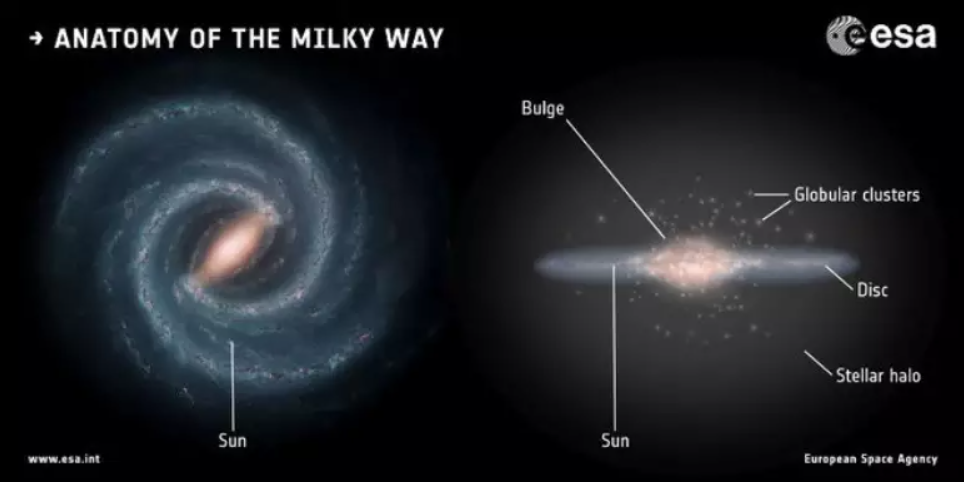
\includegraphics[width=0.8\textwidth]{Imagens/esa_estrutura_galaxia.PNG} 
  \caption[Componentes de uma galáxia espiral.]{Nesta imagem temos um exemplo dos componentes de uma galáxia espiral, como a nossa galáxia, Via Láctea. O bojo (bulge) possui uma grande densidade de estrelas e pode ser alongado ou arredondado; o disco (disc) possui estrelas, predominantemente jovens, que seguem uma onda de densidade responsável pela característica espiral; o halo é composto por gás interestelar pouco denso, estrelas mais velhas, aglomerados globulares e matéria escura. Créditos: NASA/JPL-Caltech e ESA/ATG medialab.} 
  \label{fig:esa_estrutura_galaxia} 
\end{figure}

Mas, como surgem as galáxias e como evoluem? Mesmo que ainda discutido, acredita-se que locais com alta densidade de matéria escura e instabilidades gravitacionais podem favorecer a formação de galáxias \cite{2018sm}. Há duas hipóteses que surgiram na segunda metade do século passado sobre a origem e evolução das galáxias: a monolítica e hierárquica \cite{2022gastao}. No modelo monolítico, as galáxias teriam se formado e evoluído de forma isolada e pelo colapso de grandes nuvens de gás em contração, e dependendo das condições iniciais, densidade e \emph{momentum} angular da nuvem, diferentes tipos de galáxias surgiriam. Já no modelo hierárquico, as primeiras galáxias teriam se originado nos poços de potencial criados pela concentração de matéria escura, e as galáxias maiores e massivas, através de interações e fusões entre si. Contudo, alguns pontos em relação à formação de algumas estruturas continuam em estudo \cite{2018sm}, em virtude de que há semelhanças entre galáxias com histórias evolutivas possivelmente diferentes, tornando necessário o desenvolvimento de teorias que descrevam a acumulação de matéria para a origem destes objetos. Durante o processo de formação de uma galáxia, conforme a riqueza de matéria bariônica (matéria formada por átomos de elementos conhecidos) também, elas apresentarão propriedades diferentes umas das outras \cite{2018cdf}. 

Em 1936, \citeonline{hubble1936} descreve importantes análises e conclusões das palestras Silliman, na Universidade de Yale, e publica o livro \emph{Realm of the Nebulae}\footnote{Livro baseado no esquema proposto por John Reynolds em \emph{Photometric measures of the nuclei of some typical spiral nebulae}, em 1920.}, onde propõe uma classificação morfológica para as galáxias, conhecida como esquema de Hubble. A análise da morfologia das galáxias é importante para o estudo de sua estrutura, informações sobre a cinemática, regiões onde estrelas novas estão se formando e classificação de acordo com suas semelhanças, identificando fases evolutivas e propriedades das populações estelares (estrelas jovens e velhas).

\begin{figure}[!h]
  \centering 
  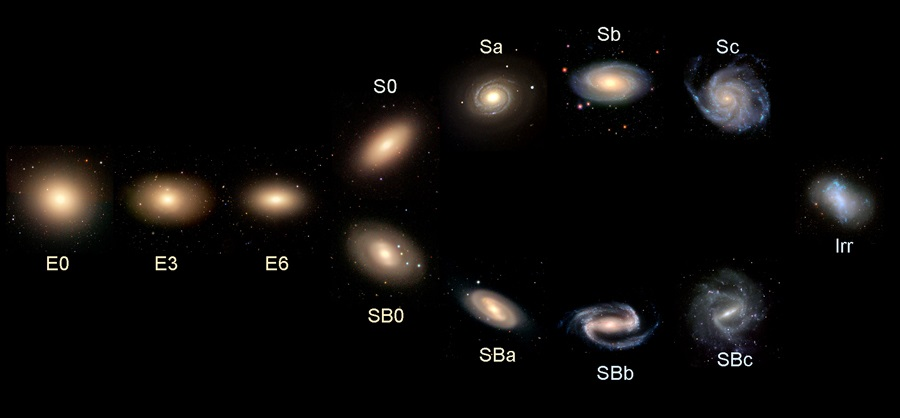
\includegraphics[width=1.0\textwidth]{Imagens/HubbleTuningFork.jpg} 
  \caption[Esquema de Hubble de classificação de galáxias.]{Representação esquemática de classificação das galáxias. Créditos: Galaxy Zoo.} 
  \label{fig:esquema_hubble} 
\end{figure}

Neste esquema (Figura~\ref{fig:esquema_hubble}), não evolutivo, pioneiro de classificação morfológica, Hubble propôs três classes de galáxias, as elípticas, espirais e irregulares. Anos seguintes, o esquema teve o acréscimo de mais duas classes, as lenticulares e espirais barradas. As galáxias elípticas (E0 a E6, Figura \ref{fig:eliptica_lenticular}) possuem formato esférico ou elipsoidal e tem como componentes o bojo e halo. A propriedade de achatamento em seu formato tendendo do circular ao elíptico é dada por E\emph{n}, em que \emph{n} é a elipticidade projetada através da orientação dos planos de simetria (\emph{n} = 10(1 - b/a), b/a sendo a razão entre os eixos menor e maior da elipse), que determina sua classificação entre E0 a E6. Uma galáxia elíptica perfeitamente circular será uma E0, enquanto uma mais plana, uma E7. Elas não possuem ``braços espirais'', e ao longo de sua estrutura, há baixas concentrações de gás, poeira e estrelas jovens.

\begin{figure}[h] 
  \centering 
  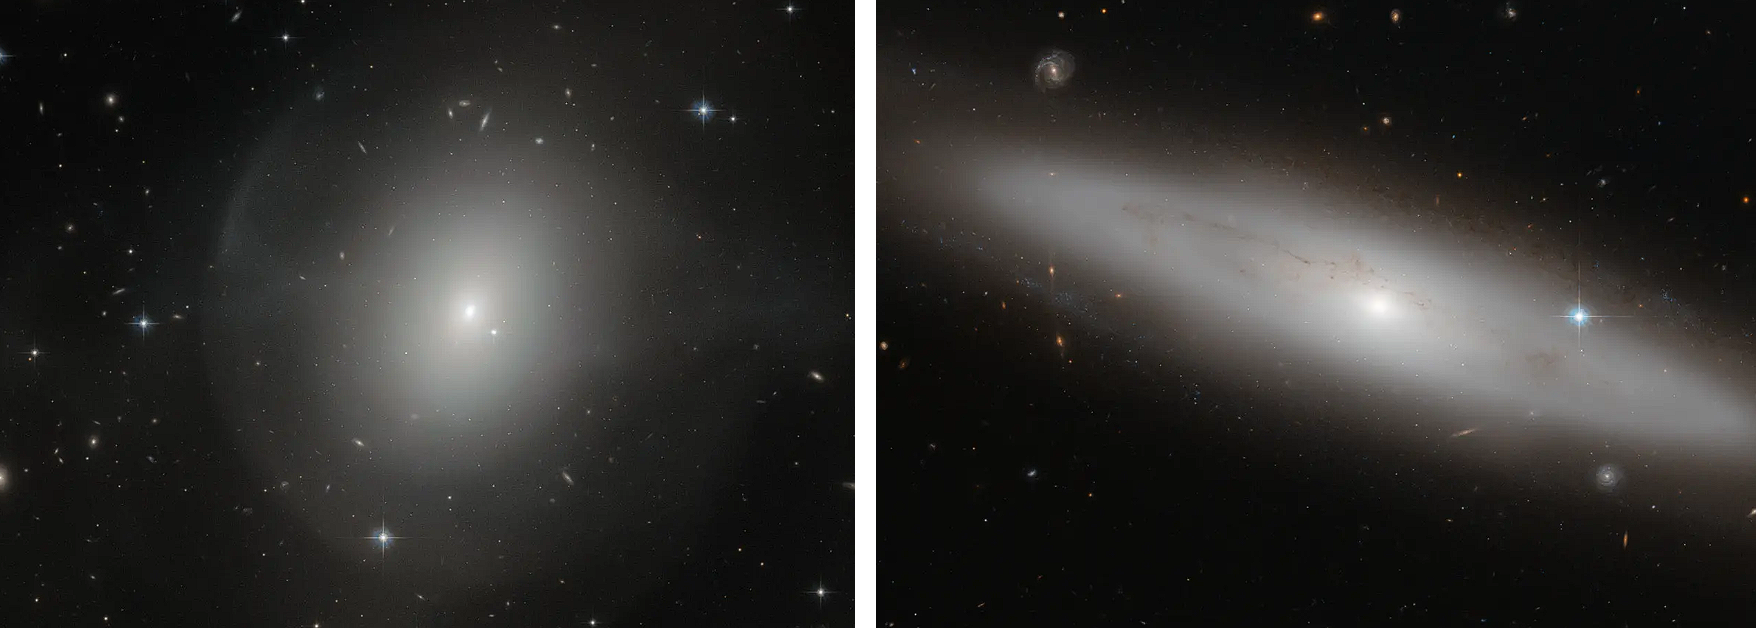
\includegraphics[width=0.8\textwidth]{Imagens/eliptica_lenticular.png} 
  \caption[Gálaxia elíptica NGC 2865 e gálaxia lenticular NGC 4886.]{A gálaxia elíptica NGC 2865, à esquerda, está localizada a 100 milhões de anos-luz de distância. A gálaxia lenticular NGC 4886, à direita, possui principalmente estrelas antigas, mas não braços espirais. Créditos: ESA/Hubble \& NASA.}
  \label{fig:eliptica_lenticular} 
\end{figure}

As elípticas possuem uma grande densidade de estrelas que diminui conforme distância do bojo, principalmente estrelas antigas, e variam amplamente em tamanho, desde as gigantes, com diâmetros de milhões de anos-luz e massas de até 10 trilhões de massas solares, até as anãs, com diâmetros de apenas alguns milhares de anos-luz. As galáxias lenticulares (S0 e SB0, Figura \ref{fig:eliptica_lenticular}) possuem morfologia intermediária entre uma elíptica e espiral, com um formato de disco (o disco, fundamental nas galáxias espirais e lenticulares, é a região plana que compõe a parte principal e mais visível da galáxia, responsável pela maior parte da massa e da atividade estelar observada), bojo com concentração de estrelas, porém com ausência de espiras \cite{2018sm,2022gastao,2023Kepler}.

As galáxias espirais (Figura \ref{fig:espirais}), quando vistas de frente (em relação ao ângulo de visada da Terra), apresentam uma clara estrutura espiral (as ``espiras'' são ondas de densidade que se propagam através do disco galáctico, compostas principalmente por estrelas, gás e poeira interestelar), diferem entre si conforme o tamanho e formato do bojo e ao nível de desenvolvimento das espiras. Estas galáxias apresentam um formato discoidal onde se estendem as espiras, halo (região estendida e difusa que envolve o disco principal da galáxia, composto principalmente por estrelas antigas, gás difuso, matéria escura e aglomerados globulares), braços espirais (onde há muitas estrelas jovens, pois à medida que o material interestelar passa por essas ondas de densidade, ele é comprimido e desencadeia a formação de novas estrelas), e bojo, podendo ser este barrado ou normal.

\begin{figure}[h] 
  \centering 
  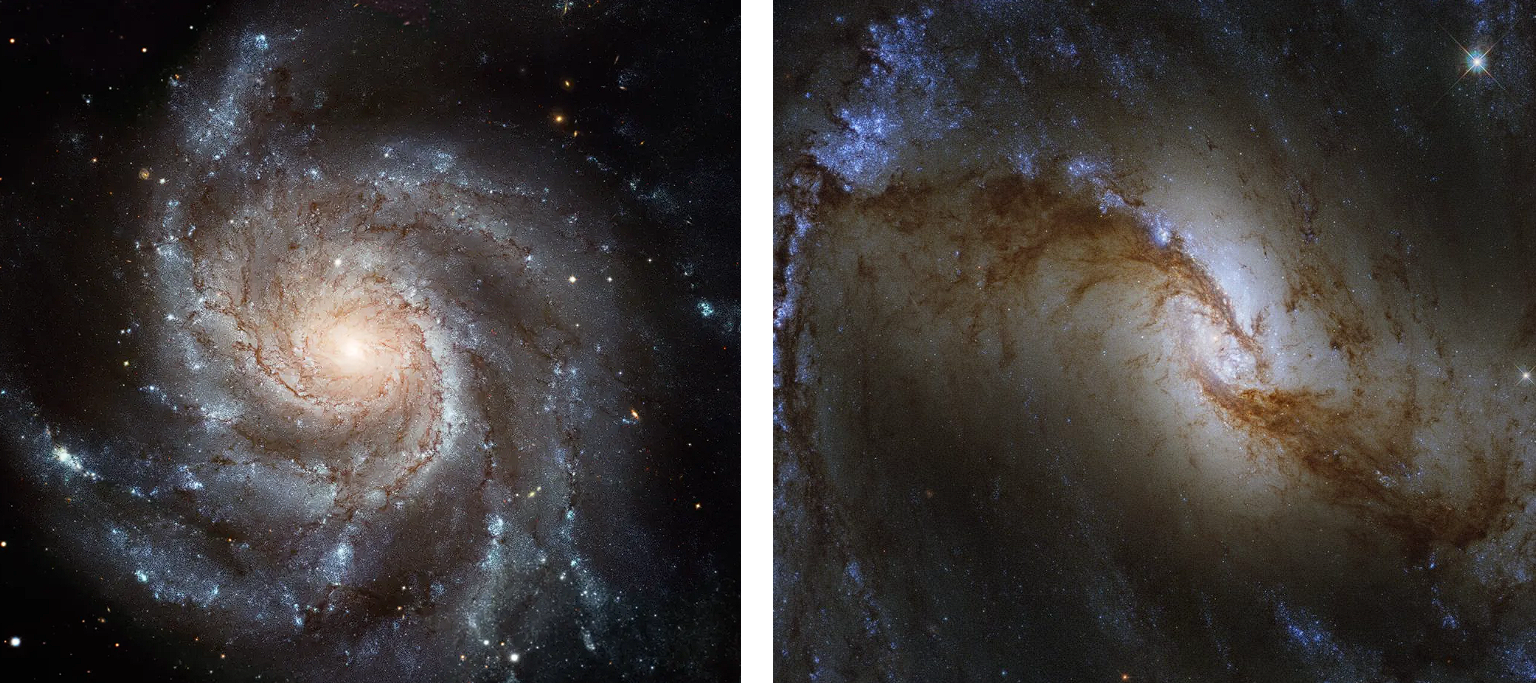
\includegraphics[width=0.8\textwidth]{Imagens/espirais.png} 
  \caption[Galáxia espiral M101 e espiral barrada NGC 1365.]{Galáxia espiral M101, à esquerda, conhecida como galáxia Pinwheel, está localizada a cerca de 27 milhões de anos-luz de distância na direção da constelação Ursa Maior. Créditos: Hubble Image: NASA, ESA, K. Kuntz (JHU), F. Bresolin (University of Hawaii), J. Trauger (Jet Propulsion Lab), J. Mould (NOAO), Y.-H. Chu (University of Illinois, Urbana) e STScI; CFHT Image: Canada-France-Hawaii Telescope/J.-C. Cuillandre/Coelum; NOAO Image: G. Jacoby, B. Bohannan, M. Hanna/NOAO/AURA/NSF. A galáxia espiral barrada NGC 1365, à direita, localizada na constelação de Fornax, possui fortes colorações azuis, regiões onde estrelas acabaram de se formar. Créditos: ESA/Hubble \& NASA.}
  \label{fig:espirais} 
\end{figure}

Galáxias espirais normais (Sa a Sc), possuem núcleo com formato esférico (comum) e suas espiras partem tangencialmente desse núcleo em posições opostas. Por exemplo, uma galáxia Sa é uma espiral com núcleo grande e braços espirais pequenos, bem enrolados, de difícil resolução. Por outro lado, as galáxias Sb têm braços espirais mais soltos, o núcleo é de tamanho moderado, menor do que o das Sa, e contêm mais gás e poeira, promovendo uma maior formação estelar. As galáxias Sc apresentam braços espirais muito soltos e proeminentes, núcleo pequeno e menos luminoso, e o conteúdo de gás e poeira é alto, favorecendo a formação de muitas estrelas novas \cite{2023Kepler,2022gastao}. Galáxias espirais barradas (SBa a SBc) apresentam um núcleo estruturado em forma de ``barra'' (estrutura alongada) e braços espirais, que comumente, partem das extremidades da barra. A segmentação de \emph{a} a \emph{c} segue a lógica anterior: SBa possuem braços espirais bem apertados e uma barra proeminente; SBb braços espirais moderadamente soltos e uma barra bem definida; e SBc braços espirais muito soltos e uma barra relativamente menor em proporção ao tamanho da galáxia. Geralmente se observa nos braços das galáxias espirais, o material interestelar, como nebulosas gasosas, poeira, e estrelas jovens (responsáveis pela tonalidade azulada) \cite{2023Kepler}. Ao analisar a idade das estrelas mais velhas em galáxias elípticas, observa-se que elas possuem, aproximadamente, a mesma idade das estrelas mais velhas das galáxias espirais, concluindo que ambos os tipos de galáxias tenham se originado na mesma época, quando a idade do universo era próxima de 1 bilhão de anos \cite{2023Muller}, e não uma sequência evolutiva espiral-elíptica. O que determina a característica das estrelas de uma galáxia elíptica, predominantemente mais velhas, é que estas galáxias, em sua ``juventude'', tenham formado suas estrelas em um curto período de tempo, consumindo rapidamente grande parte de seu gás, enquanto que nas espirais, a taxa de formação estelar teria sido mais demorada, preservando parte de seu gás, e portanto, promovendo a criação de novas estrelas por mais tempo. Hubble chamou as galáxias elípticas de ``primitivas'' e as espirais de ``tardias'' \cite{2022gastao, 2010arnab}.

O quinto tipo morfológico de galáxias, inclusive bem diversificado, são as irregulares (Irr). Como o próprio nome define, estas galáxias possuem uma estrutura peculiar, e geralmente, encontram-se junto a outras galáxias.

\begin{figure}[!h] 
  \centering 
  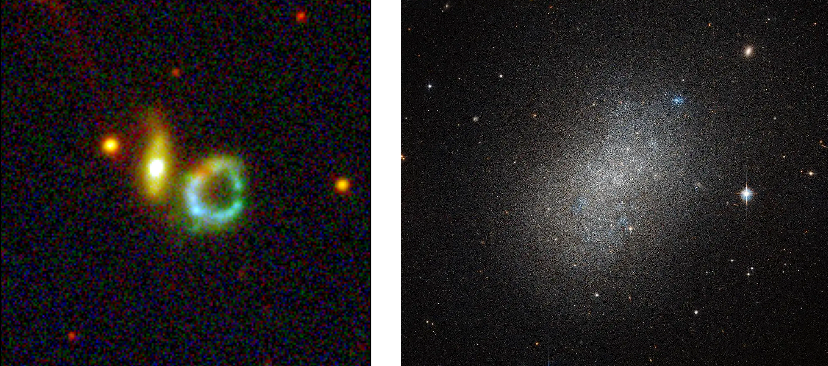
\includegraphics[width=0.8\textwidth]{Imagens/irregulares.png} 
  \caption[Gálaxia ARP 147 e gálaxia NGC 5264.]{A gálaxia irregular ARP 147, à esquerda, peculiar do tipo anelada. Crédito: Southern Photometric Local Universe Survey. A gálaxia NGC 5264, à direita, irregular e anã. Créditos: ESA/Hubble \& NASA.}
  \label{fig:irregulares} 
\end{figure}

As galáxias irregulares (Figura \ref{fig:irregulares}) apresentam uma distribuição de luminosidade sem um padrão, nuvens de gás ionizado distribuídas irregularmente, geralmente intensa taxa de formação estelar, e são classificadas em dois tipos, Irregular I e Irregular II. O tipo Irr I, é o mais comum dos sistemas irregulares, possuem riqueza em gás e muitas estrelas jovens, enquanto que Irr II tem maior quantidade de poeira, são mais raras e vermelhas \cite{2009soares, 2022gastao}.

Essas morfologias irregulares podem ser provocadas por perturbações, deformações e interações gravitacionais, como colisões (galáxia-galáxia), distorções das marés e canibalismo galáctico (fusão) \cite{2023Muller, 2022gastao}, como ilustra a Figura \ref{fig:interações}.

\begin{itemize}
	\item Colisões: As colisões entre galáxias são mais frequentes em aglomerados do que em regiões menos densas. Essas colisões potencialmente provocam mudanças na estrutura das galáxias interagentes, aumento de formação estelar e atividade nuclear, podendo ocorrer de forma lenta (galáxias que se movem mais lentamente - velocidade orbital menor) resultando em uma fusão, ou rápida  (galáxias que se movem mais rápido - velocidade orbital maior) provocando perturbações morfológicas \cite{2023Muller}.
	\item Efeito de maré: Tende a deformar as galáxias que passam próximas entre si, puxando material galáctico, alongando-as, e a distribuição do material ao longo da interação é em parte, reflexo da conservação do momento angular (rotação) das galáxias antes do choque. Esse material, composto por poeira, gás, matéria escura e estrelas, dependendo, pode ser arrancado de uma galáxia (efeito \emph{tidal stripping}), se estendendo em formato de filamento, que se denomina caudas de maré \cite{2023Kepler, 2023Muller}. 
	\item Fusão: Refere-se à interação entre galáxias de tamanhos semelhantes em que uma incorpora o material da interagente, modificando sua estrutura. No entanto, quando uma galáxia maior interage com uma menor, as forças de maré da maior podem destruir a menor, processo chamado de ``canibalismo galáctico'' \cite{2023Muller}.
\end{itemize}

\begin{figure}[!h] 
  \centering 
  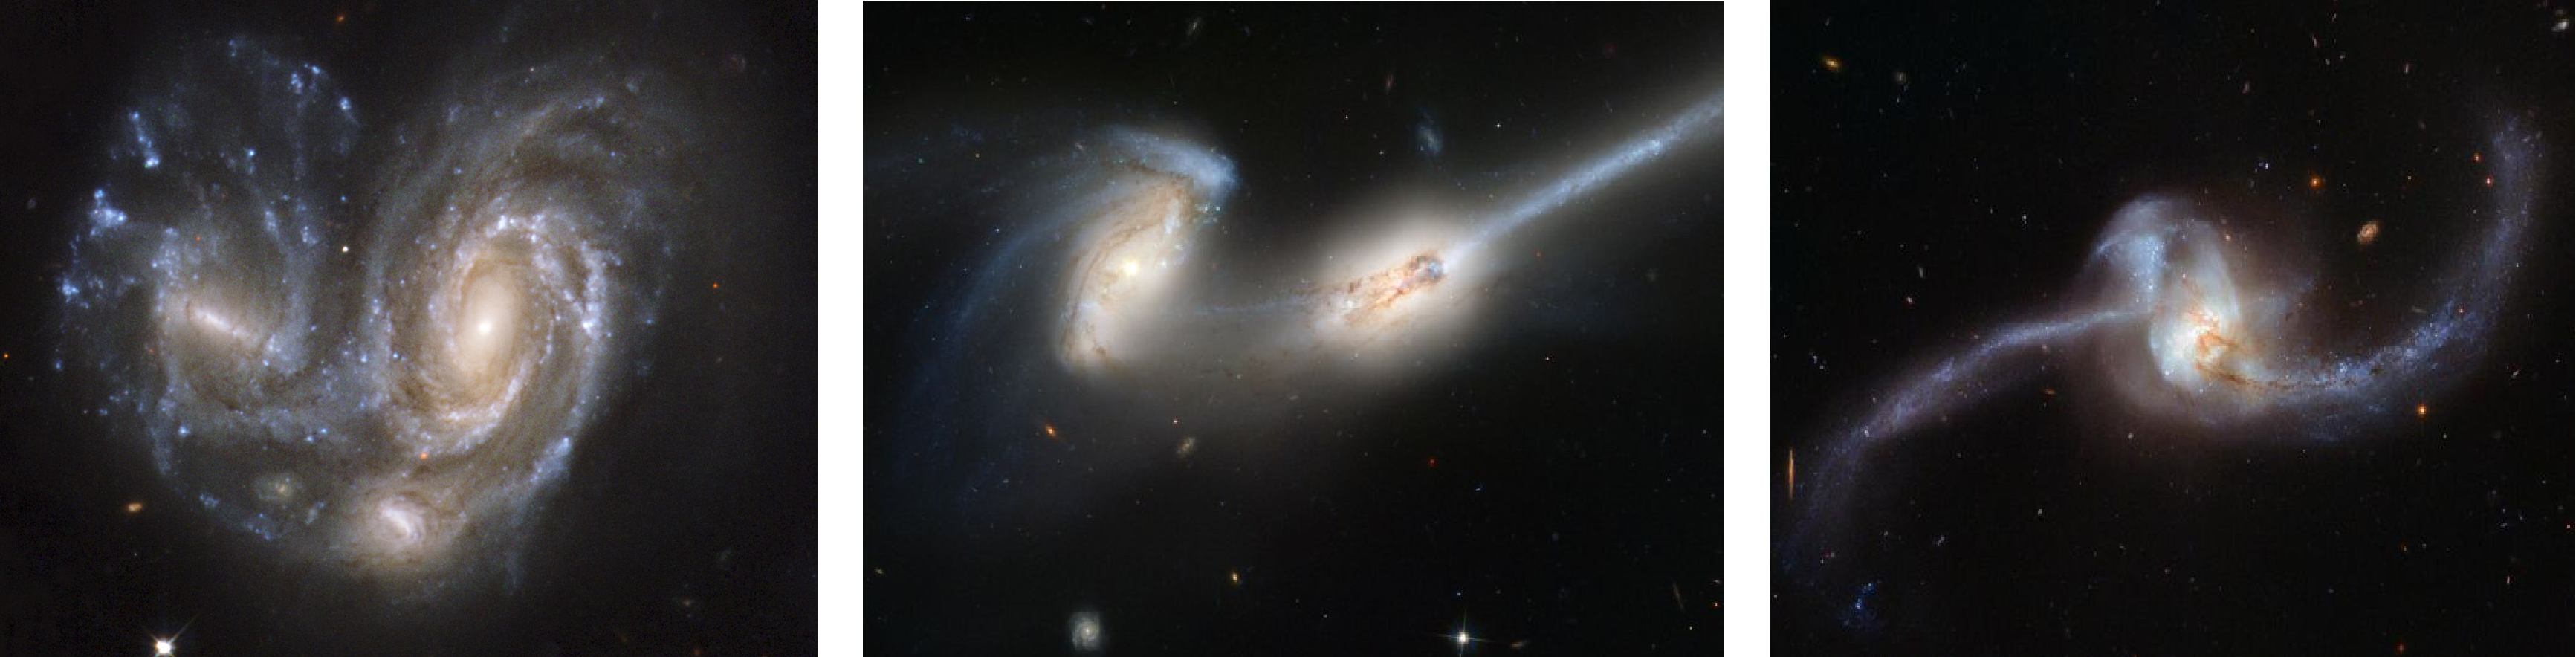
\includegraphics[width=1.0\textwidth]{Imagens/int_08.png} 
  \caption[Interação entre galáxias.]{Esquerda à direita: Colisão: NGC 6050 e IC 1179 são duas galáxias espirais que pelo processo de colisão, estão ligadas pelos seus braços espirais. Créditos: NASA, ESA, the Hubble Heritage (STScI/AURA) Hubble Collaboration, and K. Noll (STScI); Efeito de maré: observa-se as caudas longas de maré criadas nas galáxias espirais NGC 4676A e NGC 4676B, pela diferença relativa entre as forças gravitacionais nas partes próximas e distantes de cada uma. Créditos: ACS Science \& Engineering Team, NASA Hubble Space Telescope; Fusão (ou merger): NGC 2623 se encontra no estágio final da fusão, onde se observa grande taxa de formação estelar pelas cores das estrelas e também o efeito das caudas de maré estendidas. Créditos: ESA/Hubble e NASA.}
  \label{fig:interações} 
\end{figure}

Durante o processo evolutivo, ocorrem colisões de vários tipos entre galáxias. Grupos e aglomerados de galáxias são influenciados pela força gravitacional dos componentes próximos, o que pode levar à fusão das galáxias, formando galáxias gigantes. As interações entre as galáxias podem também direcionar grande quantidade de gás para a região central, propiciando a criação de um buraco negro (objeto extremamente compacto resultado do colapso de uma estrela massiva devido à força de sua própria gravidade) \cite{2003Wuensche}. Existem algumas galáxias que possuem um núcleo galáctico ativo (AGN), onde uma quantidade significativa de energia é emitida a partir de uma região compacta no centro da galáxia, que não são estrelas ou poeira interestelar, mas processos envolvendo buracos negros supermassivos, que absorvem gás de estrelas vizinhas, liberando energia potencial na forma de radiação. Elas são divididas em quasares, rádio-galáxias, blazares e Seyfert, de acordo com sua aparência e natureza da radiação que emitem \cite{2022gastao}. Os quasares, ou fontes de rádio quase-estelares, são objetos extremamente luminosos e distantes no universo, considerados como galáxias jovens que têm no seu centro buracos negros com massas de 1 milhão a 1 bilhão de vezes a massa do Sol \cite{2023Muller}.

\begin{figure}[!h] 
  \centering 
  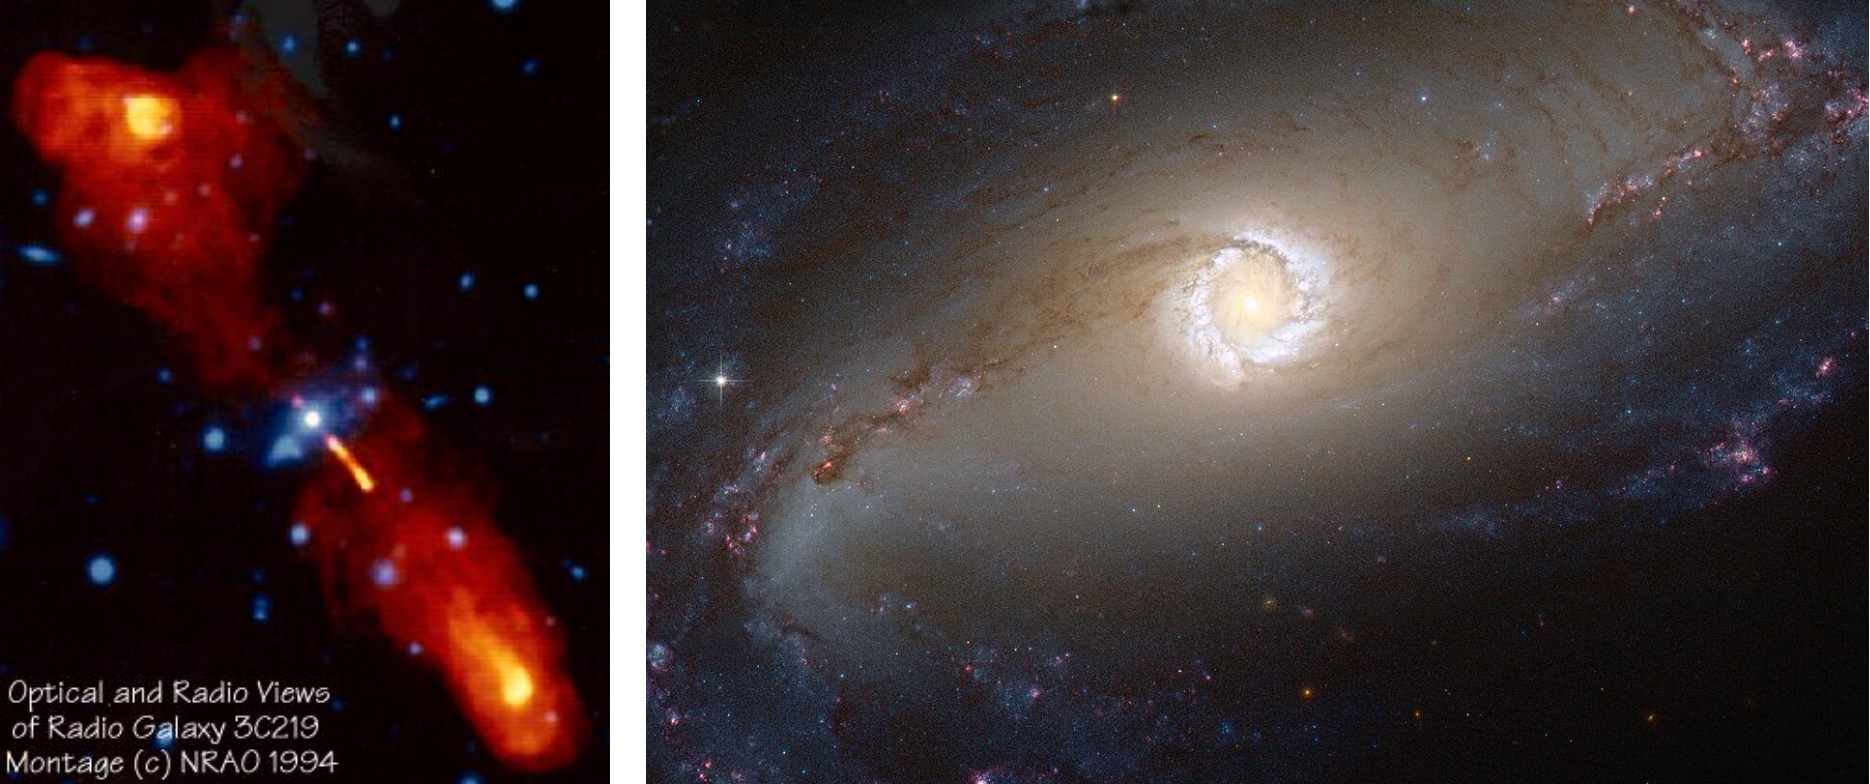
\includegraphics[width=1.0\textwidth]{Imagens/agns.png} 
  \caption[Exemplos de galáxias com núcleo ativo.]{Esquerda: Combinação da imagem ótica (em azul) com a rádio (em vermelho) do quasar 3C 219. Observa-se os lóbulos de matéria saindo da fonte (região central) e o forte jato em uma das extremidades do objeto. Créditos: National Radio Astronomy Observatory. Direita: A galáxia NGC 1097 é um exemplo de Seyfert. O buraco negro supermassivo no centro tem o equivalente a 100 milhões de massas solares. Créditos: ESA/Hubble \& NASA; E. Sturdivant.}
  \label{fig:} 
\end{figure}

A luminosidade intensa dos quasares pode ser devido a  contração do gás que sobrou após o processo de formação da galáxia, estrelas supermassivas girando a enormes velocidades e possuindo um campo magnético intenso (conhecidas como spinars) ou mesmo buracos negros gigantescos no núcleo de uma galáxia, especialmente em forma de luz visível, raios-X, e rádio (a Figura \ref{fig:espectro} exibe os tipos de luz (radiação eletromagnética)) \cite{2003Wuensche}. As rádio-galáxias, semelhante aos quasares, são galáxias que emitem grandes quantidades de ondas de rádio, geralmente têm a aparência de uma galáxia elíptica grande, mas, observadas em rádio, apresentam uma estrutura dupla com dois lóbulos emissores, que são grandes estruturas de matéria, podendo ser maiores que a própria galáxia hospedeira. Outra característica das rádio-galáxias é a presença de um jato de matéria que sai da fonte central localizada no núcleo da galáxia \cite{2003Wuensche,2010arnab}. As galáxias Seyfert são galáxias espirais com núcleos muito brilhantes, mais comuns e menos luminosas que os quasares, e a emissão de radiação dessas galáxias tende a variar em períodos relativamente curtos, sugerindo que a fonte é compacta, como um buraco negro supermassivo. Os blazares, ou BL Lac, são galáxias com jatos apontados diretamente para a Terra, exibindo intensa variabilidade e núcleo brilhante. Muitos desses objetos são fontes de rádio, logo, acredita-se que são rádio-galáxias, porém orientadas de forma que a linha de visada fica na direção do jato \cite{2022gastao}. 

\section{Galáxias peculiares aneladas}

As galáxias irregulares, ao contrário das galáxias espirais e elípticas que possuem estruturas mais definidas, não têm uma forma regular, geralmente, caóticas e assimétricas, e para algumas, locais de intensa atividade de formação estelar \cite{2023Muller}. Nesta pesquisa temos como foco um dos tipos de galáxias irregulares, as galáxias que possuem anéis. As galáxias aneladas, RGs (ring galaxies) ou ``galáxias em anel'', têm a aparência de um anel, e conforme \citeonline{Appleton96}, são frutos de acidentes cósmicos de proporções gigantescas. Uma das primeiras galáxias aneladas apresentadas foi a \emph{Cartwheel}\footnote{Identificação de outros catálogos: AM 0035-335, ESO 350-40 e HRG 35002.} (Figura~\ref{fig:cartwheel}), localizada na constelação do Escultor, descoberta pelo astrônomo suíço Fritz Zwicky, em 1941. As RGs, geralmente, têm seu núcleo localizado em uma posição assimétrica em relação ao anel e podem possuir estruturas como nódulos nos anéis, i. e. regiões que têm alta taxa de formação estelar, filamentos e deformações \cite{2016lago}. 

O astrônomo americano Halton Arp publicou em 1966 o \emph{Atlas of peculiar galaxies} \cite{1966Arp} que contém 338 imagens de galáxias do hemisfério norte, agrupadas de forma a reunir objetos com estruturas exóticas e semelhantes. A classificação das galáxias aneladas foi feita pela primeira vez por \citeonline{1976ApJ...208..650T}, com base no catálogo de Arp (1966), denominando-as por R (do inglês \emph{ring}). Em 1987, \emph{A catalogue of southern peculiar galaxies and associations} \cite{1987arpmadore} categorizou 489 galáxias peculiares do hemisfério sul, em 25 tipos morfológicos, sendo a sexta categoria, as RGs. O estudo desses objetos nos auxilia a compreender alguns dos processos de perturbações e interações entre as galáxias, e também, nos confrontar com outros que não compreendemos.

Os anéis, comumente azuis comparados a outras galáxias normais, possuem condensações de regiões HII (hidrogênio ionizado), onde há atividade de formação estelar intensa \cite{2011fogarty}. Estudos mais precisos dos anéis, e casos particulares, são necessários para certificar que constituem de fato toda a galáxia e que realmente têm forma de anel no espaço, e não conchas esféricas ou um efeito de absorção de matéria peculiarmente distribuída \cite{Agosto1970}, para desta forma obter uma caracterização de propriedades das RGs e classificar qualitativamente suas morfologias de acordo com classes e sub-classes. Pesquisas com dados fotométricos \cite{2024MNRAS.527.2816M, 1999A&A...351..860M} mostram que os anéis possuem formação estelar intensa, e em algumas RGs, o anel é o único lugar onde estas novas estrelas estão se formando. Os anéis podem ser usados para ilustrar os efeitos da força potencial gravitacional da galáxia alvo, bem como mecanismos que levam ao nascimento e morte de estrelas na propagação de ondas de densidade \cite{Appleton96}, ferramentas para a compreensão da estrutura e evolução galáctica.

\begin{figure}
  \centering 
  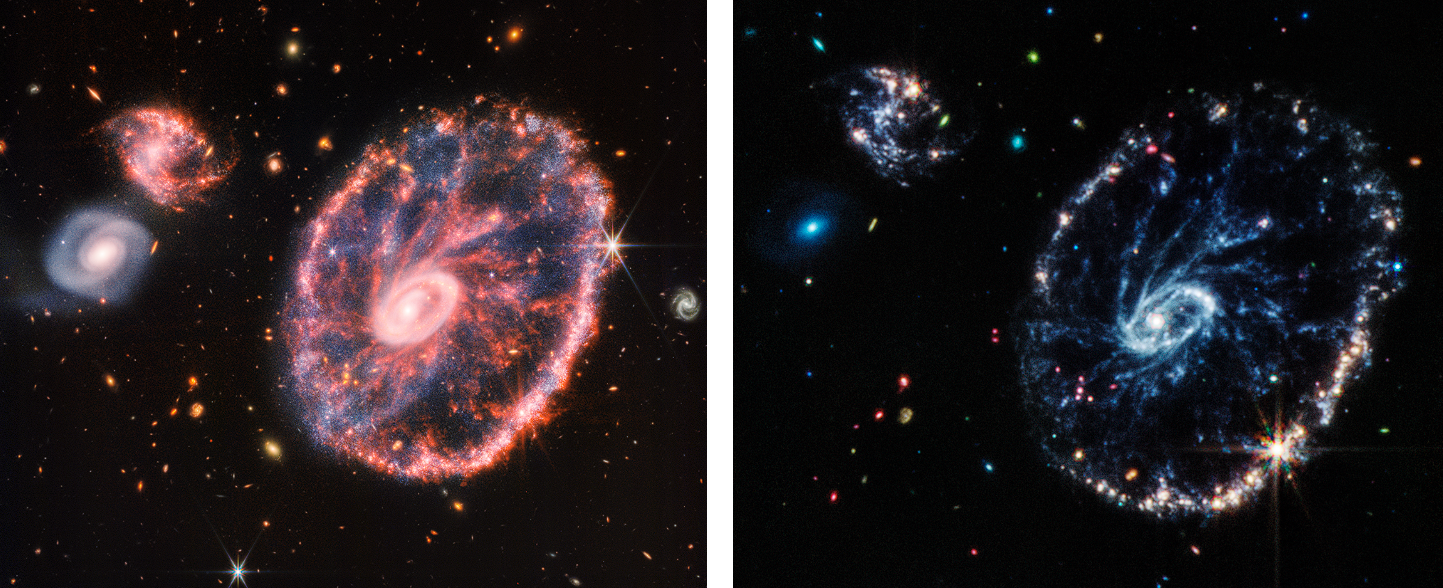
\includegraphics[width=0.8\textwidth]{Imagens/Cartwheel03.PNG} 
  \caption[Gálaxia Cartwheel.]{Esquerda: imagem no infravermelho próximo (NIRCam) e infravermelho médio (MIRI), detalhando os brilhantes anéis, interno e externo, da Grande Cartwheel. Direita: imagem no infravermelho médio (MIRI) onde se observa grande taxa de formação estelar no anel externo, enquanto que na região central há maior concentração de poeira e aglomerados de estrelas. Imagens capturadas pelo Telescópio Espacial James Webb. Créditos: NASA, ESA, CSA, STSci. O astrônomo Zwicky ao observar Cartwheel com uma câmera Schmidt de 18 polegadas na montanha Palomar em 1941, disse que esta galáxia representava "uma das estruturas mais complicadas que aguardam explicação com base na dinâmica estelar".}
  \label{fig:cartwheel} 
\end{figure}

\subsection{Morfologia peculiar}

A morfologia peculiar das RGs pode ser classificada por dois processos: quando os anéis são fruto de interações com o meio ou com outras galáxias, denomina-se como peculiares (peculiar ring galaxy - PRG) e estes objetos são bem raros, aproximadamente um a cada $10^\text{4}$ \cite{1987bin}; ou quando a origem do anel se deve a ressonância da barra de uma galáxia espiral ou perturbações do fluxo de gás do interior da galáxia, são classificados como ressonantes (normal ring galaxy - NRG), observado em galáxias SB(r), Sa(r) e SAB \cite{1998abans, 1995Buta}. Na maioria dos casos de NRG, o anel interno possui mesma idade, composição química e cor da galáxia. Anteriormente, por \citeonline{1986Madore}, foi proposta uma classificação semelhante, tipo-O para as RGs com anéis ressonantes, e para os anéis clássicos colisionais, tipo-P. Os anéis também foram classificados por três tipos de fenômenos distintos por \citeonline{1995Buta}: normal ou de ressonância, que se forma por ação de torques gravitacionais; de colisão, se origina por uma onda de choque expansiva do gás através da colisão com uma galáxia companheira; e polar, onde o anel consiste em um disco inclinado ao plano de uma galáxia, sendo fruto de uma fusão disruptiva. Atualmente, a melhor classificação morfológica das classes e subclasses das RGs é a de \citeonline{1998abans}, que categorizaram visualmente 489 PRGs do catálogo “Catalogue of Southern Peculiar Galaxies and Associations” de \citeonline{1987arpmadore}, e dividiram os anéis em cinco famílias, ilustradas na Tabela~\ref{tab:minha_tabela} e Figura~\ref{fig:quadro}: 

\begin{table}[h]
  \centering
  \begin{tabular}{ccc}
    \toprule
    \textbf{Famílias de Anéis} & \textbf{Código} & \textbf{Estruturas básicas} \\
    \midrule
    Polar & P & (a) Spindle; (b) Saturn; (c) Worm-like \\
    Hoag & H & (a) Hoag; (b) Hoag-like \\
    Elíptico & E & (a) Nódulos; (b) Suave; (c) Solitário \\
    Irregular & I &  \\
    Centralmente Suave & CS &  \\
    \bottomrule
  \end{tabular}
  \caption{Classificação dos anéis\protect\footnotemark.}
  \label{tab:minha_tabela}
\end{table}
\footnotetext{Tabela adaptada de \cite{1998abans}.}

\begin{figure}[t]
  \centering 
  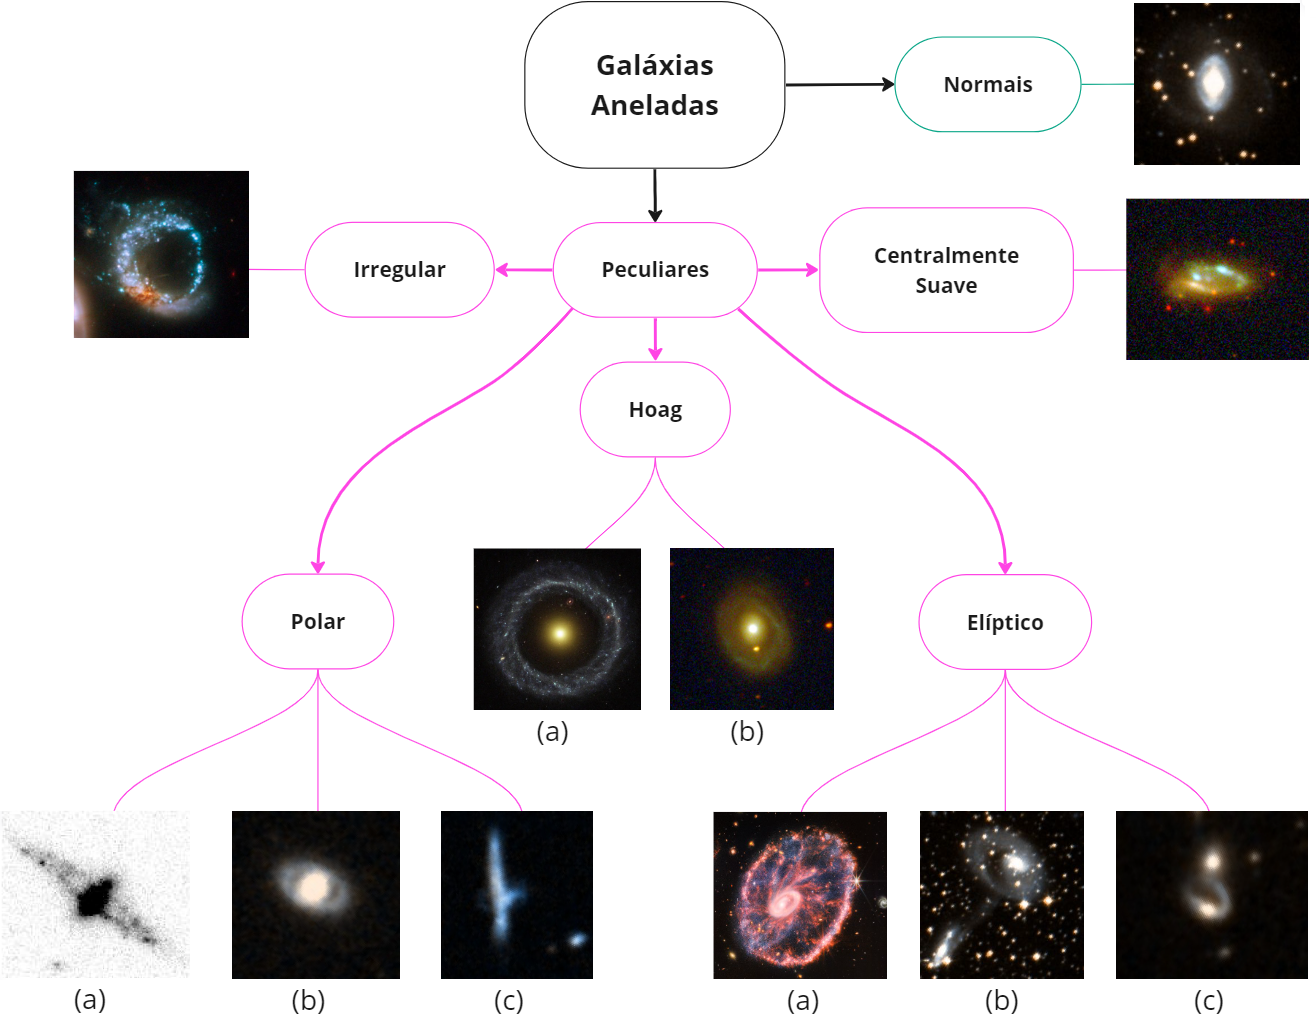
\includegraphics[width=1.0\textwidth]{Imagens/quadro.png} 
  \caption[Família dos anéis]{Polar (a) Spindle: A0136 0801, créditos: \cite{1995AIPC}; Polar (b) Saturn: HRG 54103, Polar (c) Worm-like: ESO 199-IG12, Elíptico (b) Suave: HRG 13801, Elíptico (c) Solitário: ESO 189-2, créditos: Digitized Sky Survey, STScI/NASA e CDS; Centralmente Suave: HRG 50201, Hoag (b) Hoag-like: AM 0425-421, créditos: S-PLUS; Elíptico (a) Nódulos: HRG 35002, crédito: NASA, ESA, CSA e STScI; Hoag (a): PGC 54559, crédito: NASA, R. Lucas e STScI/AURA; Irregular: ARP 147, créditos: NASA's Hubble Space Telescope. Diagrama adaptado pela classificação de \citeonline{1998abans} e construído pela autora.}
  \label{fig:quadro} 
\end{figure}

Esta divisão de classes e subclasses feita por \citeonline{1998abans}, está relacionada com as características e mecanismos de formação dos anéis, de acordo com o tamanho e formato, elipticidade e presença de um bojo no interior do anel ou nele próprio. A estrutura dos anéis do tipo Polar são resultado da acreção ou fusão de matéria rica em gás de uma companheira próxima. À estas RGs da família Polar, são atribuídas três estruturas básicas: Spindle (fuso ou eixo alongado), que possui anel em forma de fuso e perpendicular (ou quase) ao eixo da galáxia; Saturn (Saturno), galáxia com núcleo (bojo) esférico ou elíptico e anel redondo; Worm-like (tipo minhoca), contém um bojo alongado semelhante a uma minhoca e anel com nódulo (região de forte formação estelar) \cite{1998abans}. Os objetos da família Hoag, o nome vem de Arthur Hoag, astrônomo americano que descobriu em 1950 uma RG nomeada posteriormente de objeto de Hoag (galáxia PGC 54559), possuem um notável anel circular ao redor do bojo e são divididos em dois tipos: Hoag, o anel possui simetria circular e um bojo difuso; Hoag-like (semelhante ao Hoag), possui anel difuso e bojo característicos de baixa elipticidade ou bojo esférico grande comparado ao Hoag. Os anéis classificados como elípticos, são mais alongados como o formato de uma elipse e subdivididos em: com nódulos, regiões de intensa formação estelar e o bojo se encontra um pouco deslocado do centro do anel; suave, o gás que constitui o anel se distribui de forma suave em torno do bojo; e solitário, quando o núcleo (bojo) da galáxia se encontra no anel (anel com um único nódulo). As RGs categorizadas com anéis irregulares, possuem o formato pseudo-anéis ou anéis vazios com nódulos, sem um bojo localizado na região central do anel ou deslocado, e à família dos anéis centralmente suaves, são galáxias em forma anelada com nódulos e de aparência difusa, em que não se encontra uma protuberância ou bojo definidos. Alguns exemplos de galáxias das classes de NRG e PRG são ilustradas na Figura~\ref{fig:quadro}. O estudo das galáxias aneladas peculiares, que representam, em todos os casos, interações passadas ou em andamento \cite{1983AJ}, traz informações importantes dos processos interativos em escala galáctica que ocorrem no Universo, permite a observação do berçário de estrelas nos anéis, a dinâmica e trilhas evolutivas estelares.

\subsection{Estudo dos processos interativos}

Em 1950 quando o astrônomo Hoag estudava o objeto PGC 54559, achava que provavelmente seria uma nebulosa planetária ou um fenômeno de lente gravitacional (anel de Einstein), porque na época não tinham imagens ou observações detalhadas suficientes para calcular a distância do anel e do núcleo (bojo) para afirmar que estavam à mesma distância e que portanto, seriam tudo o mesmo objeto. Em 1987, \citeonline{1987sch} confirmaram que tanto o anel circular brilhante quanto o núcleo de PGC 54559 estavam à mesma distância e que constituíam uma galáxia como um todo, apresentando observações fotométricas e espectroscópicas. Na década de 70, \citeonline{1976ApJ...208..650T} realizaram um estudo de propriedades observacionais básicas sobre a estrutura de um conjunto de RGs, onde sugerem que, em sua maioria, o anel se forma devido a uma perturbação gravitacional na galáxia hospedeira, possibilitando o estudo da dinâmica galáctica entre os objetos interagentes. \citeonline{1972ApJ...178..623T} e \citeonline{1976ApJ...209..382L}, realizaram simulações computacionais numéricas de perturbações gravitacionais (exemplos de simulações são representados nas Figuras \ref{fig:simulacao} e \ref{fig:simulacaotmtm}), para entender a formação dos anéis através da colisão de uma nuvem ou galáxia com outra galáxia, em geral, através do seu centro.

\begin{figure}[h]
  \centering 
  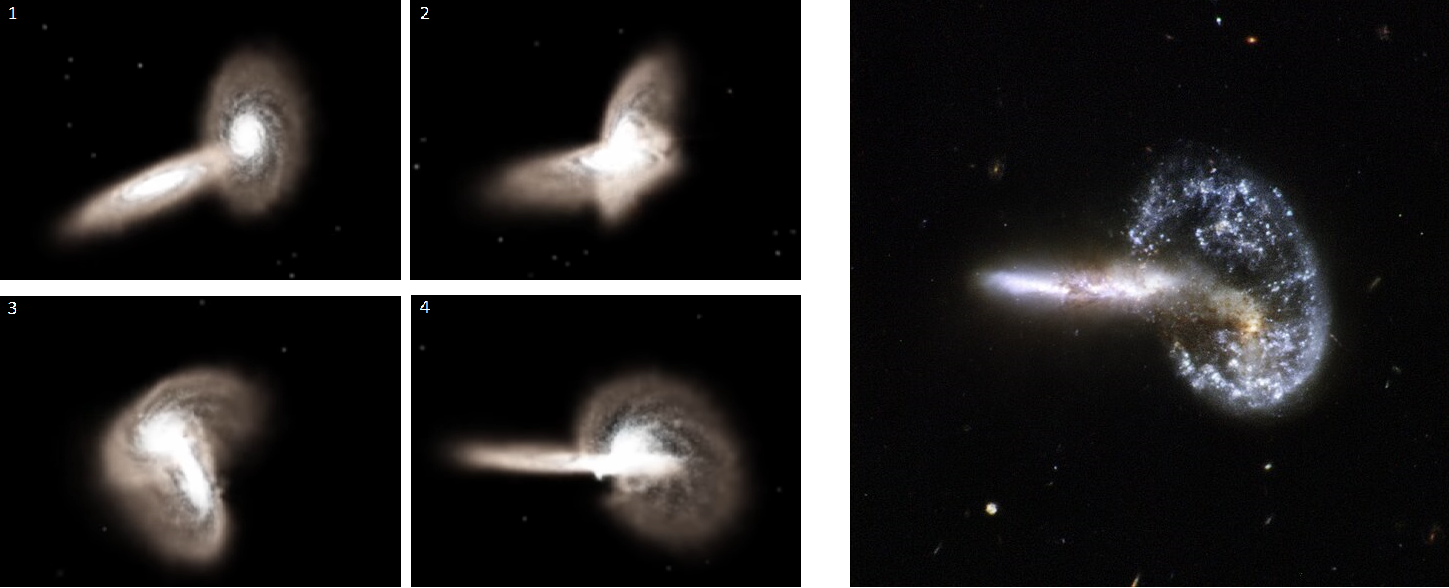
\includegraphics[width=0.8\textwidth]{Imagens/simuvsobs.png} 
  \caption[Simulação vs. Observação.]{Esquerda: simulação da interação entre duas galáxias espirais. Crédito: Summers, 2008. Direita: galáxia ARP 148. Créditos: NASA, ESA, the Hubble Heritage (STScI/AURA) e A. Evans (University of Virginia, Charlottesville/NRAO/Stony Brook University).}
  \label{fig:simulacao} 
\end{figure}

\begin{figure}[h]
  \centering 
  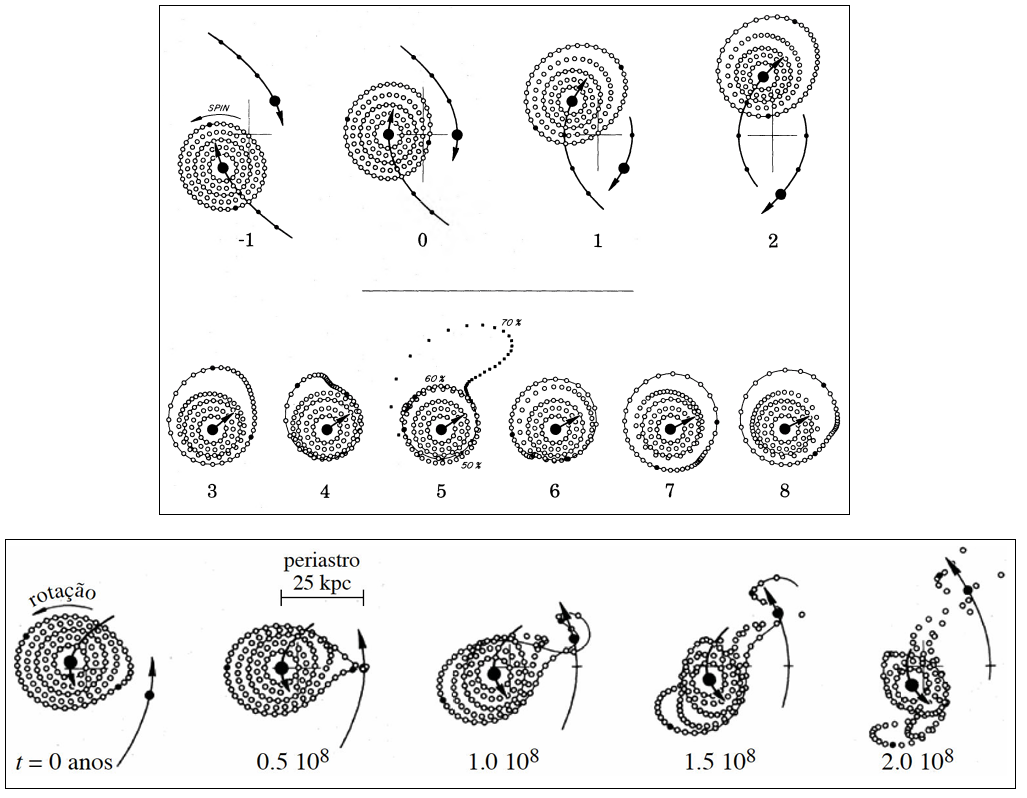
\includegraphics[width=0.8\textwidth]{Imagens/tmtmsimu.png} 
  \caption[Simulação de partículas de teste.]{Acima: Simulação da passagem de um objeto companheiro de mesma massa, onde se observam as interpenetrações parciais dos anéis mais externos e suas oscilações. Abaixo: Simulação da passagem próxima de uma galáxia anã de uma espiral. Créditos: \cite{1972ApJ...178..623T}}
  \label{fig:simulacaotmtm} 
\end{figure}

\citeonline{1974free} apresentaram um modelo para ilustrar a formação dos anéis, por meio de encontros com nuvens de HI (hidrogênio neutro) intergalácticas e as implicações para as propriedades e remanescentes dessas interações. O estudo apresenta modelos específicos de galáxias peculiares com base no conceito proposto de encontros galáxia-nuvem, em que a existência dessas nuvens moderadamente densas é postulada com base em evidências de observações de nuvens HI em vários sistemas galácticos, demonstrando que a morfologia depende da galáxia original, estágio evolutivo, ângulo de incidência e velocidade dos corpos no evento.

Atualmente, é bem reconhecido que as galáxias que passam por colisões e interações de maré intensas, resultam em fusão ou transmutação \cite{Appleton96, 2009madore}, mudando significativamente sua estrutura, e uma das possíveis consequências dessas interações, são os anéis desencadeados em discos galácticos \cite{2013A&A...558A..13F}. Muitos outros trabalhos de simulações, como por exemplo de \citeonline{2024MNRAS.528..620M}, para analisar diferentes cenários de uma colisão para a formação de uma galáxia peculiar anelada, como também pesquisas envolvendo fotometria e espectroscopia, para estudar sistemas que estão em interação ou já passaram e classificar o objeto quanto às subestruturas morfológicas encontradas \cite{1999A&A...351..860M} são fundamentais para conhecer propriedades das RGs e seu processo evolutivo.

Quando se compara as classes de galáxias aneladas peculiares Polar e Hoag, por exemplo, há uma diferença de posição do anel em relação ao núcleo da galáxia. Nas galáxias polares pode-se ver claramente em suas formas a fusão de galáxias e a força gravitacional entre elas causada pela interação, apresentando uma estrutura de anel catastrófico e o gás ``espalhado'' entorno da galáxia. Os objetos Hoag, por outro lado, estruturados como se tivessem sido formados por um processo calmo e perfeito. Em 2018, \citeonline{2018MNRAS.476.3269B} estudou modelos de potencial e movimentos de partículas de teste para Hoag's Object, observando as órbitas em torno da estrutura circular anelada. Analisou como a força entre o núcleo esférico e o anel equilibram as forças gravitacionais, e propõe, que está em uma região que denomina de OSCO\footnote{Denomina-se órbita circular estável mais interna (ISCO), onde o raio ISCO é 3Rg, (Rg = 2GM/c² é o raio de Schwarzschild). Neste caso, as órbitas estáveis estão dentro da última órbita circular estável. Por analogia, órbita circular estável mais externa (OSCO - do inglês \emph{outermost stable circular orbit}).} (Figura~\ref{fig:osco}). Este estudo mostra como o anel circular de Hoag's Object se mantém em equilíbrio e bem definido em torno da região central elíptica da galáxia.

\begin{figure}[h]
  \centering 
  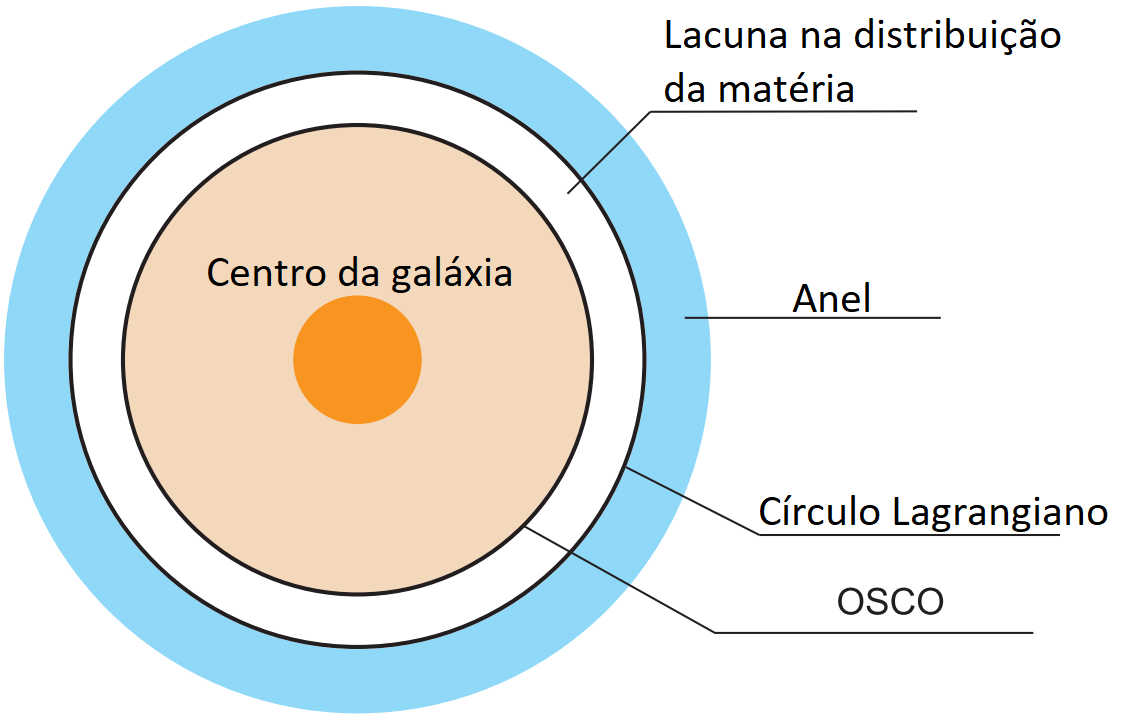
\includegraphics[width=0.95\textwidth]{Imagens/innerring.PNG} 
  \caption[Estabilidade das órbitas em sistemas de anéis do tipo Hoag.]{Esquerda: a estabilidade das órbitas em sistemas de anéis do tipo Hoag. Adaptado de \citeonline{2018MNRAS.476.3269B}. Direita: galáxia PGC 54559 de anel Hoag. Créditos: NASA, The Hubble Heritage Team (STScI/AURA) e Ray A. Lucas (STScI/AURA).}
  \label{fig:osco} 
\end{figure}

Recentemente, \citeonline{2024MNRAS.527.4112S} realizaram simulações cosmológicas TNG50 para acompanhar a formação e evolução das galáxias e traçar a origem de estruturas polares em galáxias de anel polar, e sugerem que estas estruturas são o resultado da estreita interação entre a galáxia hospedeira e sua companheira e que podem aumentar a atividade nuclear da galáxia central e/ou desligar completamente o núcleo ativo.

\begin{figure}[h]
  \centering 
  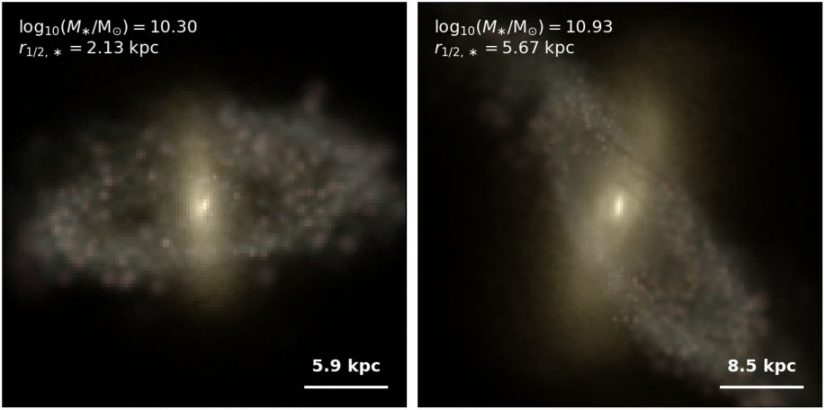
\includegraphics[width=1.0\textwidth]{Imagens/2024prg.PNG} 
  \caption[Simulações cosmológicas de galáxias com anéis polares.]{Esquerda: imagens de candidatas a galáxias com anel polar do Illustris TNG50. O canto inferior direito indica a escala das imagens, e no canto superior esquerdo, massa estelar total e o raio de meia-massa estelar. Créditos: \citeonline{2024MNRAS.527.4112S}. Direita: galáxia NGC 660 de anel polar. Créditos: Gemini Observatory/AURA.}
  \label{fig:2024prg} 
\end{figure}

As imagens sintéticas e a distribuição de massa bariônica (Figura~\ref{fig:2024prg}) foram usadas para identificar galáxias com anéis polares na simulação. Os autores investigaram dois caminhos de formação dos anéis polares estelares: formação de estrelas no gás agregado e interrupção das marés do componente estelar do satélite, observando um aumento constante na inclinação dos anéis ao longo de bilhões de anos. As características das galáxias simuladas, como luminosidades integrais, cores e tamanhos, foram em geral, de acordo com as atuais observações.

\subsection{Observação de propriedades}

Algumas observações de RGs, como a Cartwheel e o anel Lindsay-Shapley, encontraram evidências das galáxias responsáveis pela colisão dentro da faixa de distância, velocidades e ângulos de posição, esperados para interações colisionais frontais \cite{1977MNRAS.178..473F, 2009madore}. A Figura \ref{fig:g3} é uma composição mostrando uma imagem óptica da grande galáxia Cartwheel e galáxias menores, sobreposta com observações de rádio de alta resolução do hidrogênio neutro (representado pelos contornos verdes). Observa-se a trilha de hidrogênio neutro, do gás e poeira em ondas de rádio, mapeando sua distribuição e identificando a galáxia na extrema direita a cerca de 250 mil anos-luz, responsável pela colisão.

\begin{figure}[h]
  \centering 
  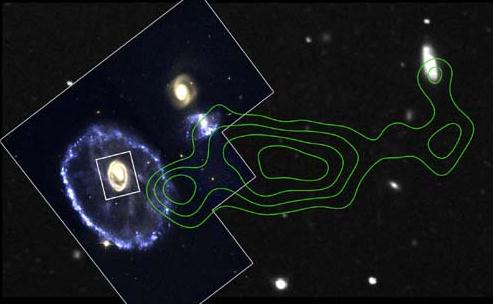
\includegraphics[width=0.8\textwidth]{Imagens/cartwheel2_hst.jpg} 
  \caption[Galáxia Cartwheel e sua interagente.]{A grande galáxia do grupo Cartwheel sobreviveu a uma colisão com uma pequena galáxia viajante, o que fez possível a formação de um anel expansivo ao redor do núcleo galáctico. Pela imagem do Hubble vemos as regiões azuis brilhantes no anel que são grandes aglomerados de estrelas recém-nascidas. Créditos: J. Higdon (NRAO), C. Struck, P. Appleton (ISU), K. Borne (Hughes STX), R. Lucas (STScI), NASA/ESA, Hubble Space Telescope.}
  \label{fig:g3} 
\end{figure}

Nos últimos anos, houve um grande avanço no estudo em múltiplas bandas em RGs (Figura \ref{fig:cart4}), para analisar propriedades dos anéis, como a taxa de formação estelar. Em 2008, \citeonline{2008ASPC..381..128A} apresentaram resultados de um levantamento GALEX e SPITZER de RGs colisionais, com combinação de imagens e espectroscopia UV e infravermelho médio, investigando a relação entre as regiões de formação estelares massivas e o aquecimento da poeira nos anéis. Em Cartwheel, por exemplo, analisaram o desenvolvimento do anel e suas doze fontes luminosas ULXs (fontes de raio-X ultraluminosas), revelando um gigantesco disco UV externo. Os autores sugeriram que as fontes ULXs sejam coleções de binárias de raios-X de alta massa, associadas a aglomerados estelares massivos e luminosos, responsáveis pelo aquecimento da poeira no anel externo, e que as variações de FUV/NUV (ultravioleta distante e próximo) ocorrem com a absorção de poeira, conforme mapeado pelo Spitzer. Em 2012, \citeonline{prestwich2012} descobriram uma correlação entre o número dessas fontes luminosas e a taxa de formação estelar, através de simulações de população binária de raios-X de alta massa para NGC 922 e Cartwheel (ambas RGs com anel em expansão), para entender a origem de ULXs. A população ULXs nos dois objetos foi analisada, levando em consideração fatores como metalicidade (visto que ambas as galáxias possuem proporções diferentes) e taxa de formação de estrelas. As simulações previram a razão do número dessas fontes em ambas as galáxias com a taxa de formação estelar, concluindo que a metalicidade da Cartwheel não é baixa o suficiente para mostrar uma diferença na população de ULXs em comparação com NGC 922. Neste estudo, os autores propuseram também que as ULXs possam ser dominadas por sistemas com forte acreção de massa de buracos negros gigantes de colapso-direto, contribuição importante para o seu papel na evolução das galáxias. Quando estrelas massivas explodem como supernovas, deixam para trás estrelas de nêutrons e buracos negros, que podem possuir estrelas próximas e se tornarem poderosas fontes de raios-X muito brilhantes ao retirar matéria de suas companheiras. Por possuírem essas fontes ULXs espalhadas pelo anel, estas galáxias se tornam interessantes laboratórios para sondar os objetos mais pesados do universo, os buracos negros, e conforme \citeonline{2010MNRAS.406.1116P} sugeriram, a mais brilhante fonte desses raios-X, seria provavelmente, um buraco negro de massa intermediária.

\begin{figure}[h]
  \centering 
  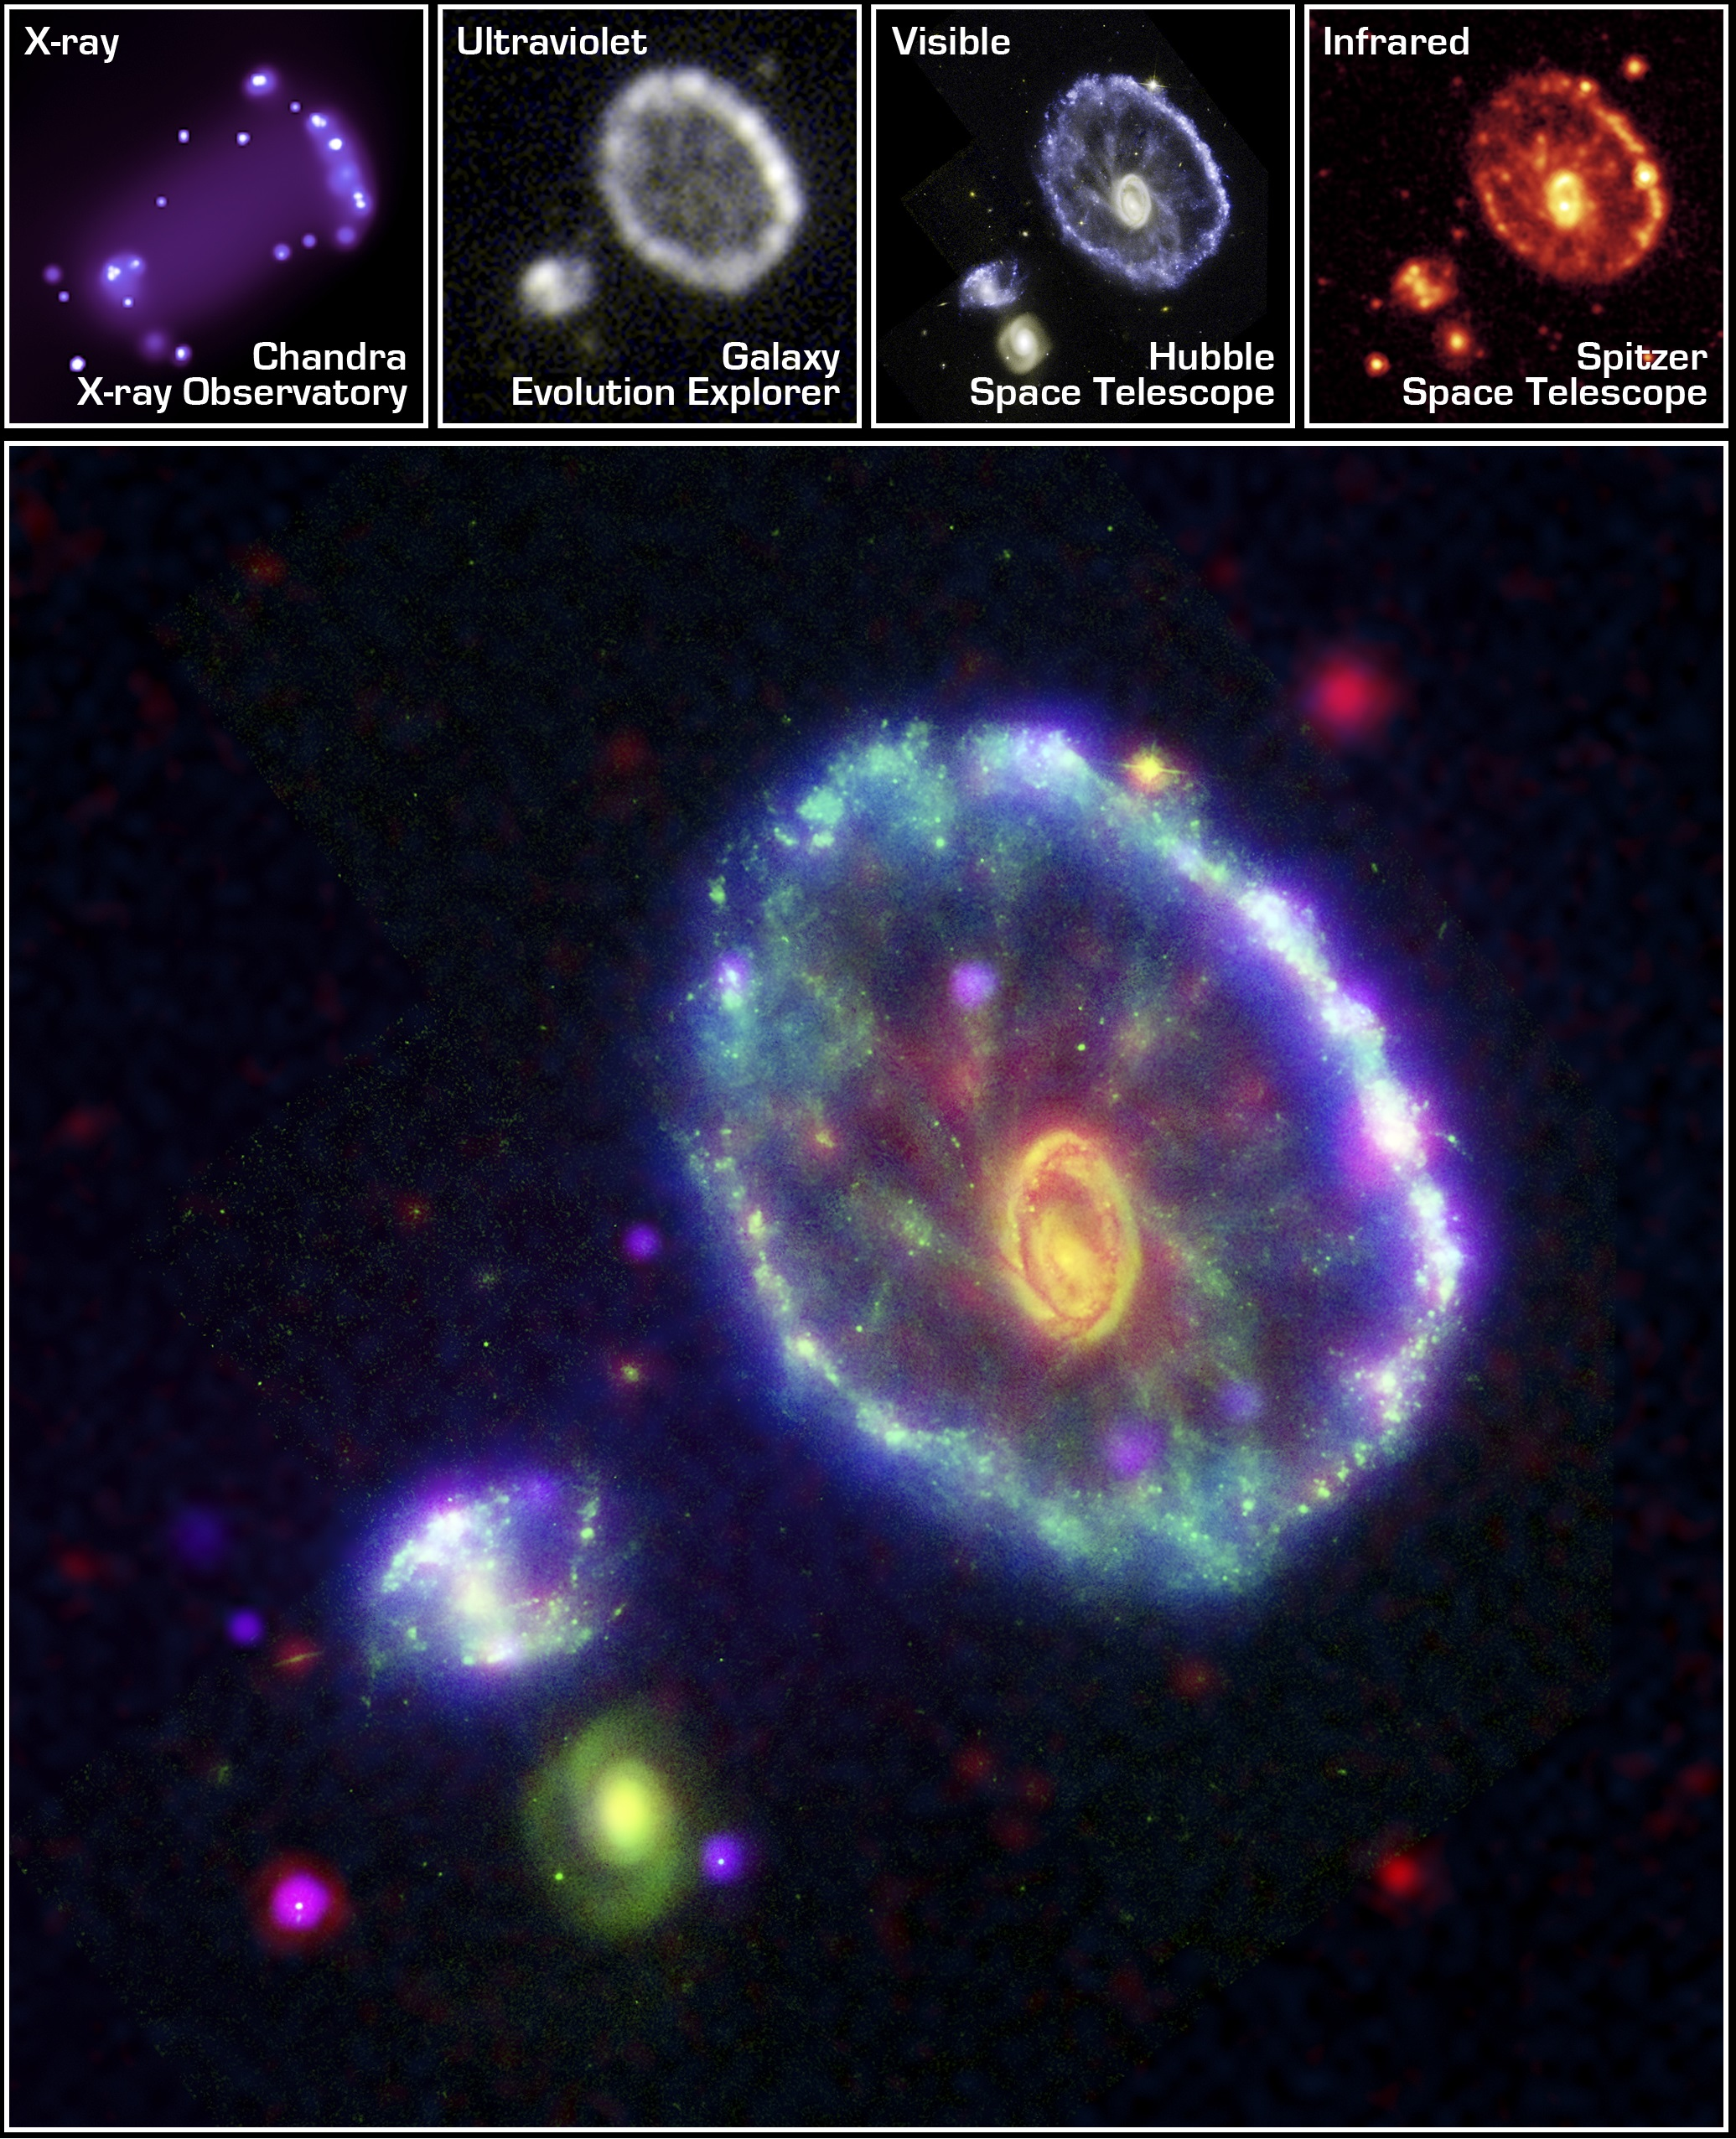
\includegraphics[width=0.65\textwidth]{Imagens/Cartwheel04.jpg} 
  \caption[Composição de imagens de Cartwheel.]{Combinação de dados de quatro observatórios: Observatório de Raios-X Chandra (roxo); satélite Galaxy Evolution Explorer (ultravioleta/azul); Telescópio Espacial Hubble (visível/verde); Telescópio Espacial Spitzer (infravermelho/vermelho). Créditos: NASA/JPL/Caltech/P.Appleton et al.; raio-X: NASA/CXC/A.Wolter \& G.Trinchieri et al.}
  \label{fig:cart4} 
\end{figure}

Evidências de estrelas jovens e velhas em Cartwheel também foram encontradas, em 2024, por \citeonline{2024MNRAS.527.2816M}, que analisaram imagens FUV (ultravioleta distante) profundas e de alta resolução obtidas com a missão AstroSat/UVIT e imagens ópticas e infravermelhas publicamente disponíveis (Figura \ref{fig:cart9}), para estudar as diferentes idades e propriedades das estrelas na galáxia. Identificaram 73 regiões no FUV, as quais 58 estão localizadas no anel externo e 15 pertencem aos ``raios'' que o ligam ao núcleo, e que há tanto estrelas antigas quando jovens no anel, sendo a maior concentração das mais velhas, no núcleo. Concluíram que, provavelmente, as regiões em UV nos raios acompanham a formação estelar desencadeada pela passagem da onda em expansão, onde algumas das estrelas formadas na onda no passado, foram arrastadas ao longo dela até a posição atual do anel, segundo o cenário colisional para galáxias aneladas.

\begin{figure}[h]
  \centering 
  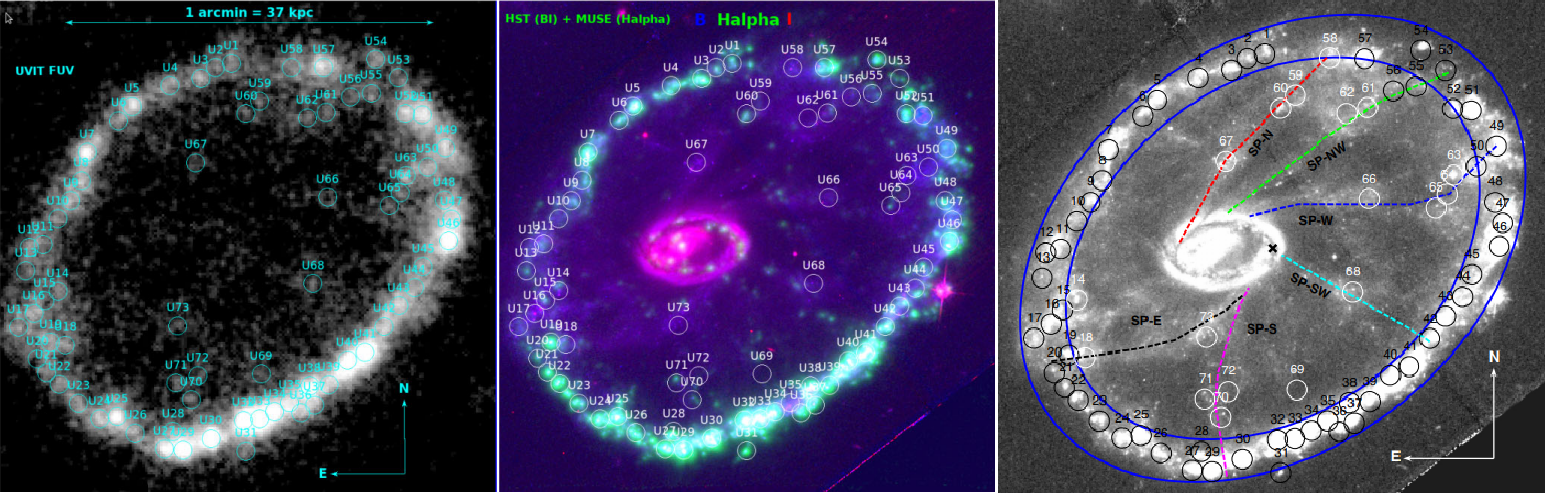
\includegraphics[width=1.0\textwidth]{Imagens/cart.PNG} 
  \caption[Galáxia Cartwheel vista com imagens no ultravioleta distante (FUV) obtidas pela missão AstroSat/UVIT, e RGB por HST/WFPC2 e VLT/MUSE.]{Esquerda: Fontes compactas FUV identificadas na imagem FUV do UVIT (círculos ciano). Meio: Imagem composta de cores RGB usando os filtros HST/WFPC2 F450W (azul), VLT/MUSE H$\alpha$ (verde) e HST/WFPC2 F814W (rosa), identificando com as cores a predominância das populações estelares I e II, no anel externo e interno, respectivamente. Direita: Identificação dos raios proeminentes na imagem F435W. Linhas tracejadas de cores diferentes são desenhadas para identificar cada raio e duas elipses concêntricas delimitam as fontes UV pertencentes ao anel formador de estrelas (círculos pretos). Todas as fontes UV situadas entre os anéis interno e externo pertencem a um dos seis raios da Cartwheel. Créditos: \citeonline{2024MNRAS.527.2816M}.}
  \label{fig:cart9} 
\end{figure}

Em 2002, \citeonline{2001MNRAS.322..689R} realizaram um levantamento de 27 galáxias de núcleos ativos, peculiares de anel polar e candidatas, e estimaram que uma porcentagem significativa da amostra eram galáxias Seyfert, cerca de 12.5-25\%, e LINERs (Low-Ionization Nuclear Emission-line Region, são galáxias que também apresentam atividade nuclear, mas em comparação com as Seyfert, têm uma ionização mais baixa em suas linhas espectrais), 33-41\%. A observação de galáxias por meio de técnicas como fotometria, que permite visualizar em imagens as diferentes estruturas, estrelas e outros componentes, e espectroscopia, que examina a interação entre a radiação e a matéria fornecendo informações sobre composição, temperatura, densidade e movimento de objetos, são fundamentais para a compreensão do funcionamento desses sistemas.

\section{Fotometria}

A fotometria é a ciência que mede a luz proveniente de um objeto, e quase toda informação que temos sobre o universo, vem na forma de luz. A luz (ou partículas que compõem a luz, os fótons\footnote{Fóton é a unidade quântica elementar de luz. Na física quântica, os fótons são descritos como partículas discretas de energia que compõem a radiação eletromagnética e têm características tanto de onda quanto de partícula.}) é uma onda eletromagnética, de campo elétrico e magnético oscilante, isto é, energia. As ondas eletromagnéticas são classificadas de acordo com seus comprimentos de onda e suas frequências, propriedades relacionadas às suas energias, quanto menor o comprimento de onda, maior a frequência e energia. O espectro eletromagnético (Figura \ref{fig:espectro}) é o intervalo completo de todas as frequências de radiação eletromagnética, abrangendo desde as ondas de rádio de baixa frequência até os raios gama de alta frequência.

\begin{figure}[h]
  \centering 
  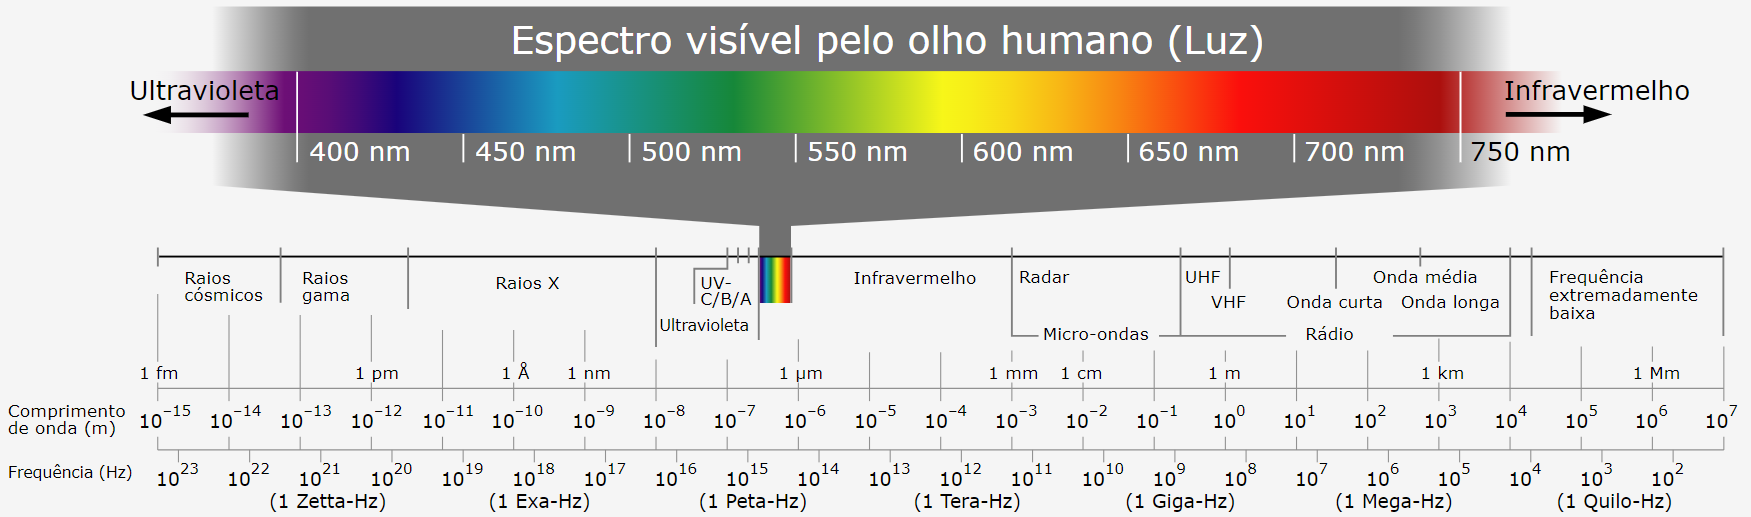
\includegraphics[width=1.0\textwidth]{Imagens/espectro.PNG} 
  \caption[Espectro eletromagnético.]{Espectro eletromagnético com todos os tipos de radiação eletromagnética que existem em nosso universo. Créditos: Horst Frank, Jailbird e Alebergen.}
  \label{fig:espectro} 
\end{figure}

A luz visível é a faixa do espectro perceptível ao olho humano, e dentro desse intervalo, diferentes comprimentos de onda correspondem às cores conhecidas. Na astronomia, a fotometria teve início no final do século XIX e, nos últimos anos, diferentes tipos de detectores nos telescópios são utilizados para estudar a radiação electromagnética do universo, invisível aos nossos olhos. Há observações astronômicas que são feitas fora da atmosfera terrestre e na superfície da Terra \cite{2023Kepler}. O espectro electromagnético, desde os raios gama até as ondas de rádio, são usados para observações astronômicas para estudar informações sobre a natureza e propriedades físico-químicas de uma fonte, como por exemplo, medir o fluxo e a cor de uma estrela e estimar sua temperatura. Para isso, é necessário usar filtros, como ilustra a Figura \ref{fig:caranguejo}, de forma que a luz de vários comprimentos de onda cheguem ao telescópio, mas somente a luz permitida pelos filtros são recebidas pelo detector.
 
 \begin{figure}[h]
   \centering 
   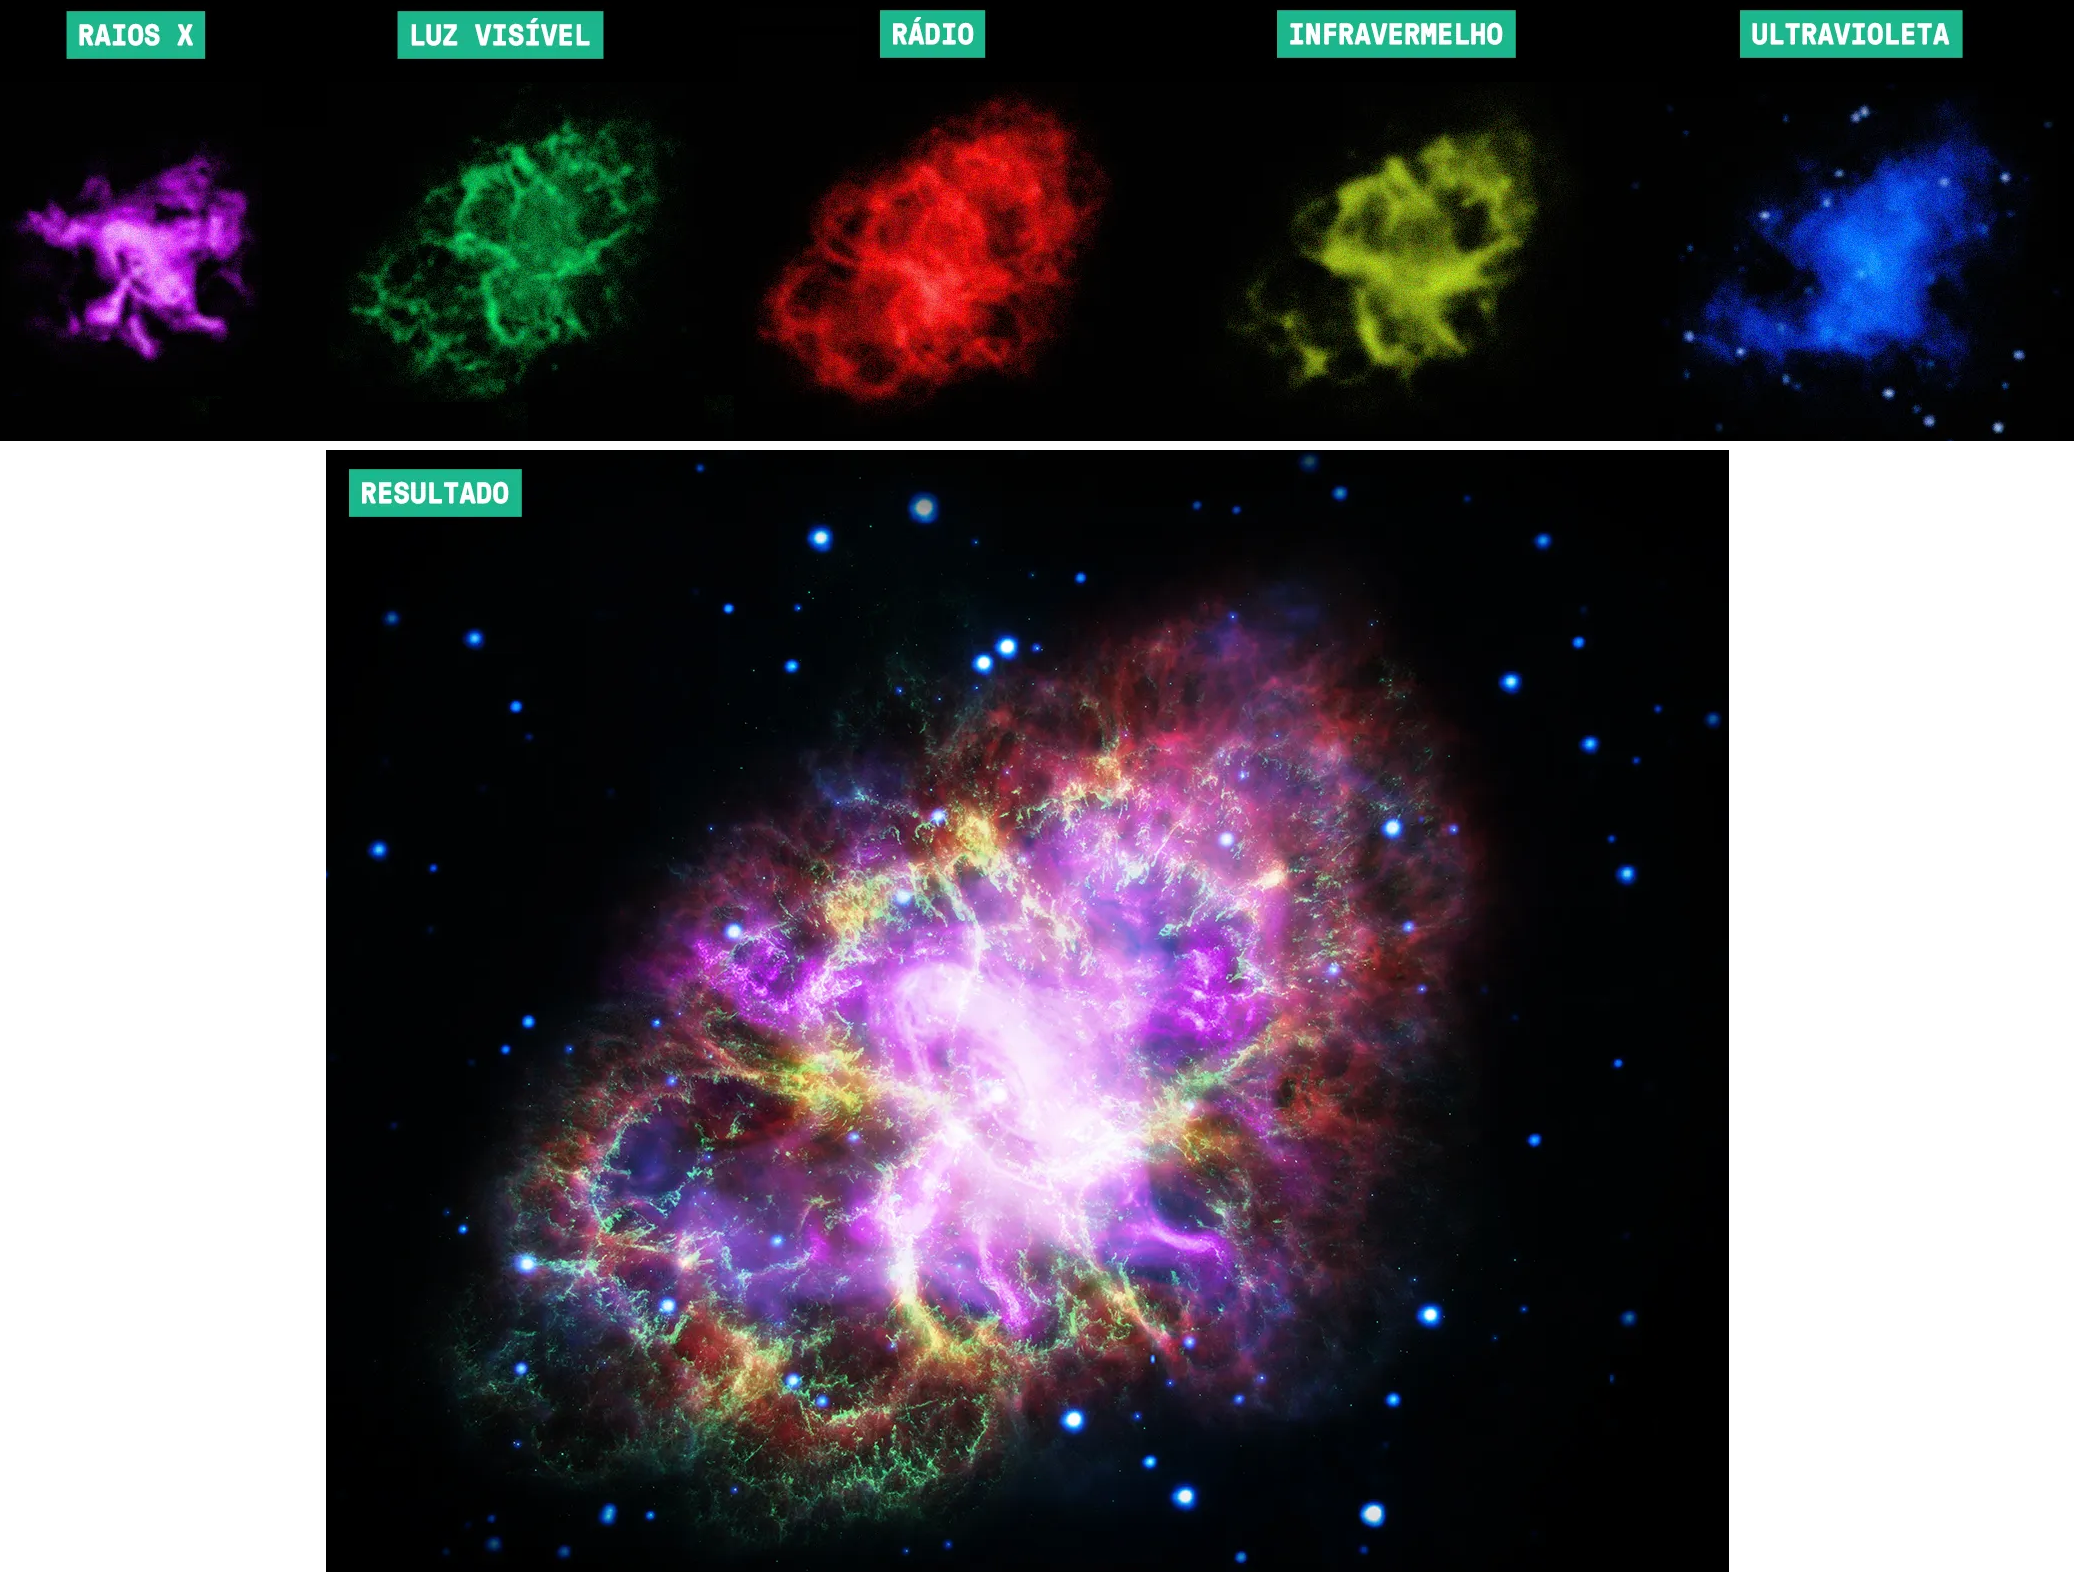
\includegraphics[width=0.83\textwidth]{Imagens/caranguejo_02.png} 
   \caption[Combinação de filtros para imagem da Nebulosa de Caranguejo.]{A Nebulosa de Caranguejo é o resultado de uma explosão de supernova, e em seu centro, há uma estrela de nêutrons super densa, emitindo luz nas ondas de rádio e visível. Na região central, há uma mistura de materiais, incluindo os que foram expelidos pela estrela antes de se tornar uma supernova e os que foram lançados durante a explosão. Ventos carregados de partículas são expelidos da estrela de nêutrons, energizando a poeira e o gás ao seu redor. Essas diversas camadas e os filamentos que compõem a nebulosa podem ser observados nesta imagem em várias faixas de comprimento de onda. Combinação de filtros: raios-X, telescópio Chandra; luz visível, telescópio Hubble; ondas de rádio, observatório Very Large Array; infravermelho, telescópio Spitzer; ultravioleta, satélite X-ray Multi-Mirror-Newton. Créditos: NASA, ESA, G. Dubner et. al., NRAO e Caltech.}
   \label{fig:caranguejo} 
 \end{figure}
 
A astronomia e astrofísica são ciências que dependem muito das observações, voltadas para imagens e processamento de imagens, portanto, os diferentes filtros representados por cores são importantes ferramentas, em uma imagem combinada de filtros e cores, e revelam, a composição química das nuvens de gás, poeira, estrelas e outros componentes de um objeto observado \cite{2007soaress}. Galáxias e nebulosas\footnote{Grandes nuvens de gás e poeira interestelar no espaço, que podem ser encontradas tanto dentro quanto fora de galáxias.} emitem mais luz em comprimentos de onda muito específicos devido aos componentes e elementos que as constituem, como o hidrogênio e oxigênio por exemplo. A quantidade de luz que recebemos de cada elemento traz informações importantes sobre a riqueza química e a física que está ocorrendo em um objeto astronômico, sendo essencial para a imagem o quanto (intensidade) dessa luz em específico existe. Para isso, é preciso cores para as bandas largas e bandas estreitas (exemplo Figura \ref{fig:narrowbandandbroadband}) para os respectivos filtros. As bandas largas cobrem uma ampla região de comprimentos de onda. Por exemplo, uma banda larga pode cobrir uma grande faixa do espectro visível ou incluir uma parte significativa do infravermelho ou ultravioleta. As bandas estreitas, são faixas de comprimento de onda relativamente pequenas, e são selecionadas para observar características espectrais específicas, como linhas de emissão ou absorção de elementos químicos, regiões de alta ionização, ou outros fenômenos que são proeminentes em comprimentos de onda específicos \cite{2023Kepler}.
 
  \begin{figure}[h]
    \centering 
    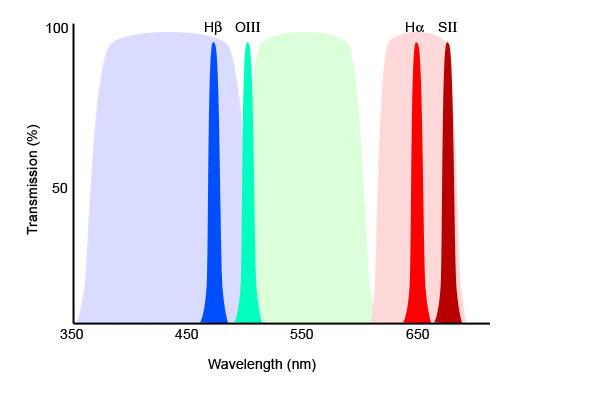
\includegraphics[width=0.7\textwidth]{Imagens/narrowbandandbroadband.jpg} 
    \caption[Exemplo de bandas estreitas combinadas com bandas largas.]{Exemplo de bandas estreitas (H$\beta$, OIII, H$\alpha$ e SII) combinadas com bandas largas (em azul, verde e vermelho claros). Créditos: tellescopio.com.br.}
    \label{fig:narrowbandandbroadband} 
  \end{figure}

Para extrair detalhes sobre os objetos observados, como as diferentes estrelas, história de formação estelar e morfológica, é necessário conhecer as emissões em cada faixa do espectro. Na faixa dos raios gama, por exemplo, podemos estudar buracos negros e regiões formadoras de estrelas, e os raios-X, observar estrelas compactas, estrelas de nêutrons e também buracos negros. A faixa do ultravioleta revela informações sobre estrelas quentes, galáxias AGNs\footnote{Galáxias que possuem regiões centrais extremamente luminosas, muito mais brilhantes do que o restante da galáxia. A intensa emissão de energia dessas regiões é causada pela presença de um buraco negro supermassivo em seu núcleo.} (galáxias de núcleos ativos) e regiões onde estrelas estão se formando. A luz visível abrange observações de planetas, estrelas, cometas, asteroides e galáxias. No infravermelho, o estudo de estrelas frias, espaço interestelar, galáxias e poeira. As micro-ondas são usadas no estudo de elementos químicos nos astros e na radiação cósmica de fundo, e as ondas de rádio, são aplicadas no estudo de quasares, rádio-galáxias e outros fenômenos \cite{2023Kepler,2022gastao}.

Em 2024, por exemplo, \citeonline {2024arXiv240412527S} realizaram fotometria no ultravioleta próximo (NUV) e ultravioleta distante (FUV) de um sistema de galáxias em interação (conhecido por Arp 298, Figura \ref{fig:ngc_ic}), composto por uma galáxia do tipo Seyfert 1, a NGC 7469, e sua companheira IC 5283, para resolver e mapear as regiões de formação estelar nos braços externos (população estelar I) e buscar sinais de interação entre as duas galáxias. Os autores derivaram a distribuição espectral de energia (SED), determinando parâmetros físicos, como a taxa de formação estelar global, massa estelar e de poeira. Esse estudo fotométrico mostrou que a maior parte da atividade de formação estelar está confinada dentro do anel central da galáxia alvo. Outro exemplo, é o trabalho de \citeonline{2024MNRAS.530.2907A}, que através da análise fotométrica, exploraram o sistema de aglomerados globulares (população estelar II) e suas propriedades na galáxia peculiar anelada polar NGC 4262 (Figura \ref{fig:ngcquiesc}). Realizaram as distribuições espaciais e azimutais das populações estelares e encontraram evidências de interações anteriores dentro da galáxia hospedeira. Além disso, investigaram as relações de escala globais entre os aglomerados globulares e parâmetros da galáxia hospedeira, dando suporte para a hipótese de que as RGs de anel polar são uma fase intermediária conectando fusões em curso e galáxias quiescentes (galáxias em que a formação de estrelas não ocorre mais de maneira significativa).

\begin{figure}[h]
  \centering 
  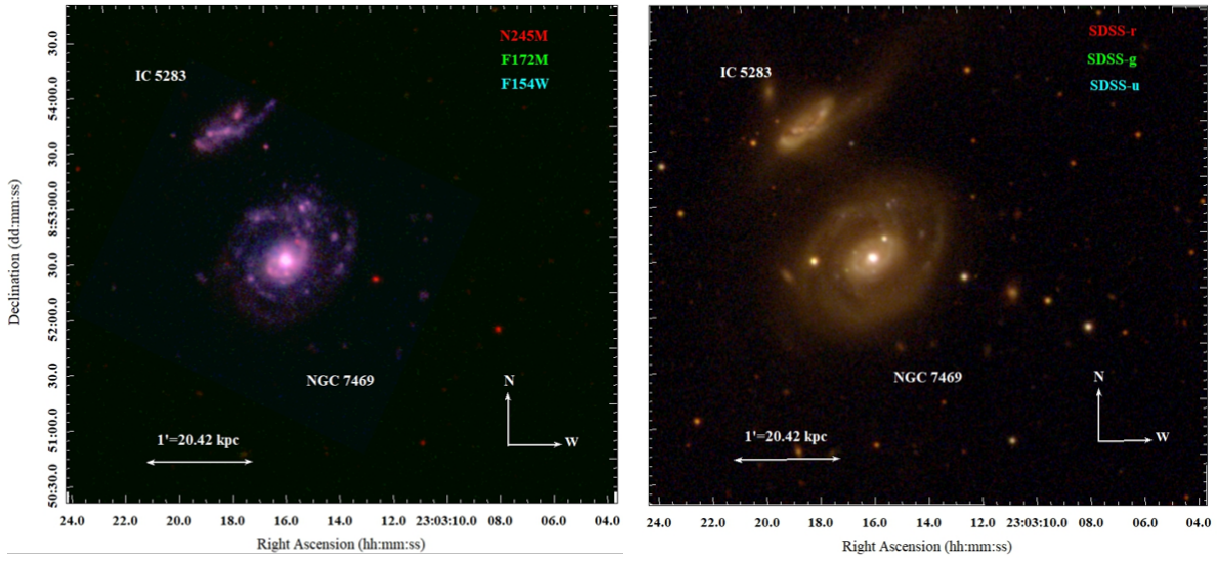
\includegraphics[width=0.8\textwidth]{Imagens/ngc_ic.PNG} 
  \caption[Fotometria das galáxias em interação NGC 7469 e IC 5283.]{Esquerda: Imagem RGB composta de NGC 7469 e IC 5283 usando os filtros N245M (vermelho), F172M (verde) e F154W (azul). Esta imagem mostra claramente a presença de braços espirais internos e nós que atuam como evidência da formação estelar. Direita: Imagem RGB composta usando os filtros SDSS-r (vermelho), SDSS-g (verde) e SDSS-u (azul). Créditos: \cite{2024arXiv240412527S}.}
  \label{fig:ngc_ic} 
\end{figure}

\begin{figure}[h]
  \centering 
  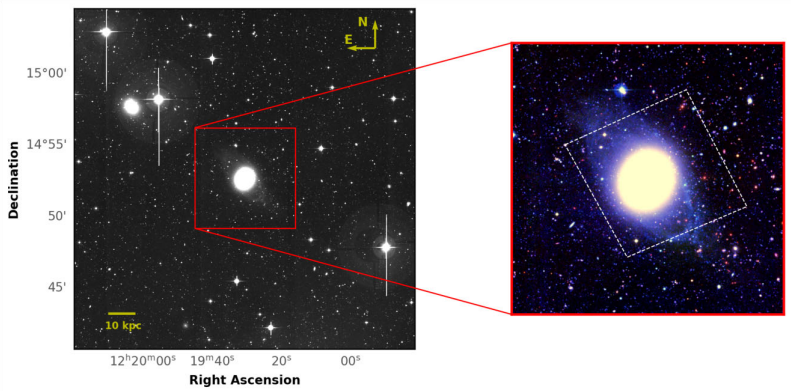
\includegraphics[width=0.8\textwidth]{Imagens/ngcquiesc.PNG} 
  \caption[Fotometria da RG polar NGC 4262.]{Esquerda: Imagem óptica em banda g de NGC4262 usando o Canada France Hawaii Telescope (CFHT). Direita: Imagem colorida óptica com as cores azul, verde e vermelho, representando as bandas CFHT u, g e i, respectivamente. Esta imagem da galáxia revela um componente de anel óptico fraco que permaneceu não detectado nas imagens ópticas anteriores. A linha pontilhada branca representa a região observada pelo Hubble Space Telescope (HST). Créditos: \cite{2024MNRAS.530.2907A}.}
  \label{fig:ngcquiesc} 
\end{figure}

O avanço científico dos levantamentos (surveys) fotométricos e espectroscópicos, antes associados aos atlas e hoje aos amplos catálogos de fontes e suas propriedades, permitem analisar e combinar informações de muitos bancos de dados, em diversos filtros para seus respectivos comprimentos de onda, e obter novas características dos objetos. Eles mapeiam a distribuição tridimensional das galáxias, aglomerados de galáxias e outras estruturas em largas escalas, de forma a ilustrar como o universo é organizado e como essas estruturas evoluíram ao longo do tempo. Ao examinar o espectro de luz, os surveys espectroscópicos revelam informações sobre a história, evolução e expansão do universo, investigando a natureza da matéria escura e da energia escura, dois dos maiores desafios da física e da cosmologia modernas. Os levantamentos fotométricos fornecem informações sobre a distribuição espacial, tamanho, forma, cor, luminosidade e outras características físicas dos objetos observados. Isso é fundamental para estudar como as galáxias se formaram, evoluíram e se enriqueceram ao longo do tempo e como interagem umas com as outras em diferentes ambientes. A fotometria de alta precisão é essencial, por exemplo, na detecção e caracterização de exoplanetas (planetas fora do nosso sistema solar). Vários programas de levantamento observacional trazem (alguns ainda em construção) imagens com grande profundidade (a grandes distâncias), para áreas extensas e com alta qualidade, como por exemplo o Dark Energy Survey (DES)\footnote{https://www.darkenergysurvey.org}, Sloan Digital Sky Survey (SDSS)\footnote{https://www.sdss.org}, Two Micron All Sky Survey (2MASS)\footnote{https://irsa.ipac.caltech.edu/applications/2MASS/IM/} e Southern Photometric Local Universe Survey (S-PLUS, detalhes na Seção \ref{sec:splus}). 

\begin{itemize}
  \item O DES é um trabalho internacional e colaborativo para, no hemisfério sul, mapear galáxias, detectar supernovas e encontrar padrões de estrutura cósmica sobre a natureza da energia escura que está acelerando a expansão do nosso universo. Possui o telescópio de 4 metros, localizado no Cerro Tololo Inter-American Observatory (CTIO) no Chile, equipado com a câmera Dark Energy Camera (DECam), com CCD de 520 megapíxeis e 2.2 graus de campo de visão, e registra imagens usando cinco filtros, abrangendo comprimentos de onda de 400 nm a 1080 nm, que correspondem respectivamente às bandas largas do SDSS \emph{griz}. O survey iniciou as pesquisas em 31 de agosto de 2013 e finalizou os dados em 2019.
  \item O SDSS é operado por uma colaboração internacional, iniciada em 2000, e tem como objetivo mapear uma grande porção do céu, utilizando uma combinação de telescópios, câmeras e espectrógrafos. Utiliza os telescópios Apache Point de 2.5 m da Fundação Sloan no Observatório, no Novo México; o telescópio Irénée du Pont de 2.5 m no Observatório Las Campanas, no Chile; e o telescópio NMSU de 1 m no Observatório Apache Point, Chile. Também utiliza os espectrógrafos BOSS, que possui duas câmeras, uma vermelha e outra azul, e uma faixa completa de comprimento de onda de 3.600 a 10.400 Å; e o espectrógrafo APOGEE, na faixa infravermelho próximo de alta resolução.O Apache Point e Irénée du Pont utilizam um sistema composto por cinco filtros, que cobrem diferentes partes do espectro eletromagnético: $u$, $g$, $r$, $i$ e $z$, centrados respectivamente em 355 nm, 468 nm, 616 nm, 748 nm, e 893 nm. O SDSS é dividido em 5 fases, cada uma focada em diferentes aspectos da astronomia. O atual SDSS-V consiste numa parceria com os Observatórios Carnegie e envolve observações nos hemisférios norte e sul. No hemisfério norte, as observações são realizadas no Telescópio da Fundação Sloan no Observatório Apache Point, no Novo México. No hemisfério sul, as observações são realizadas no Telescópio Irénée du Pont, nos Observatórios Las Campanas , no Chile.
  \item O 2MASS é um projeto astronômico que mapeou o céu em três comprimentos de onda no infravermelho próximo. Realizado entre 1997 e 2001, forneceu um levantamento detalhado, resultando em um catálogo de mais de 470 milhões de objetos. O projeto foi uma colaboração entre a University of Massachusetts e o Infrared Processing and Analysis Center (IPAC) no California Institute of Technology (Caltech), com financiamento da NASA e da National Science Foundation (NSF). Utilizou dois telescópios de 1,3 metros de diâmetro: Observatório de Monte Hopkins, Arizona, EUA, para observações do hemisfério norte; e Observatório de Cerro Tololo, Chile, do hemisfério sul; ambos possuíam três filtros infravermelhos, J (1,25 µm), H (1,65 µm) e K$_\text{s}$ (2,17 µm).
\end{itemize}

Dessa forma, é importante otimizar a detecção da radiação para a qualidade da obtenção dos dados, e atualmente, técnicas e instrumentos foram aprimorados para esta necessidade. Além disso, a qualidade da fotometria também está associada à redução de erros nos dados, que podem distorcer as análises e levar a interpretações incorretas dos espectros de energia dos objetos. O processo de fotometria envolve várias etapas para corrigir e processar as imagens capturadas pelo detector do telescópio, para que as medições finais sejam de qualidade para a análise científica. A redução de dados fotométricos consiste principalmente no tratamento de dados do detector CCD (Charge Coupled Device, ou \emph{CCD}, são circuitos que consistem de uma matriz), correção dos efeitos da atmosfera da Terra, transformação ao sistema fotométrico padrão e correção por avermelhamento interestelar. Os tratamentos de dados do CCD incluem o overscan, bias, flatfield e dark, processos responsáveis em remover efeitos aditivos e multiplicativos. Às imagens, obtidas através de diferentes filtros (ou faixas de banda), e para cada um, é medido o fluxo \cite{2023Kepler}. A qualidade dos dados fotométricos influencia diretamente a confiabilidade e a precisão das estimativas de parâmetros físicos, por exemplo, para a utilização de modelos que interpretam as distribuições espectrais de energia (SED, do inglês, \emph{Spectral Energy Distribution}) das galáxias. Dados precisos são a base para inferências sobre a formação estelar, massa estelar, atenuação da poeira e outras propriedades. Um exemplo de modelo que interpreta as SEDs de objetos é o MAGPHYS \cite{2011ascl.soft06010D}, que analisa e interpreta as propriedades físicas de galáxias com base em observações espectrais em várias faixas de comprimento de onda, desde o ultravioleta distante até o infravermelho, sendo capaz de estimar parâmetros relacionados às estrelas e ao meio interestelar das galáxias, como as histórias de formação estelar, metalicidade e conteúdo de poeira. Estas ferramentas que interpretam a SED de um objeto, comparam as distribuições de energia espectral observadas com um conjunto de modelos teóricos, com a finalidade, por exemplo, de compreender os processos evolutivos das galáxias e a investigação das propriedades do meio interestelar.

\section{Motivação e objetivos}

Esta pesquisa pretende fornecer pontos importantes sobre a qualidade da fotometria de galáxias irregulares, com ênfase na família das galáxias peculiares aneladas. Para isso, analisamos 117 objetos do hemisfério sul do universo local, a partir da base de dados de catálogos e atlas disponíveis, e encontradas no Southern Photometric Local Universe Survey (S-PLUS). No capítulo 2, discutimos sobre a ciência das aberturas fotométricas elípticas do S-PLUS utilizadas, explorando suas propriedades e como elas são usadas para a análise de dados, além de detalhar a obtenção das amostras e as metodologias de classificação utilizadas. No capítulo 3, são apresentados os resultados iniciais sobre a qualidade fotométrica das aberturas aplicadas a estas galáxias de morfologia irregular, como a diferença de leitura das magnitudes e os respectivos erros, e no capítulo 4, as conclusões e contribuições de nosso estudo, abrindo novas perspectivas para pesquisas futuras.